\documentclass{article}

\usepackage{amsmath}
\usepackage{amsfonts}
% \usepackage{CJKutf8}
\usepackage[usenames, dvipsnames]{color}
\usepackage{booktabs}
\usepackage{fancyhdr}
\usepackage{graphicx}
\usepackage{hyperref}
\usepackage{multirow}
\usepackage{pgfplots}
\usepackage{skak} %
\usepackage{tabularx}
\usepackage[thinlines]{easytable} %
\usepackage{tikz}
\usepackage{times}
\usepackage[shortlabels]{enumitem}
\usepackage{placeins}
\usepackage[title]{appendix}

\usetikzlibrary{arrows.meta}

%

\definecolor{darkgreen}{RGB}{0, 125, 0}
\definecolor{orange}{RGB}{255, 125, 125}

\newcommand{\todo}[1]{{\color{orange}{TODO: #1}}}

\newcommand{\muzero}{\emph{MuZero}}
\newcommand{\reanalyze}{\emph{MuZero Reanalyze}}
\newcommand{\alphazero}{\emph{AlphaZero}}
\newcommand{\alphagozero}{\emph{AlphaGo Zero}}
\newcommand{\alphago}{\emph{AlphaGo}}
\newcommand{\stockfish}{\emph{Stockfish}}
\newcommand{\elmo}{\emph{Elmo}}

\newcommand{\expect}[1]{\mathbb{E}\left[ {#1} \right]}
\newcommand{\expectx}[2]{\mathbb{E}_{#1}\left[ {#2} \right]}
\newcommand{\dd}[2]{\frac{\partial{#1}}{\partial{#2}}}

\definecolor{colorwin}{RGB}{156,255,161}
\definecolor{colordraw}{RGB}{220,220,255}
\definecolor{colorloss}{RGB}{255,161,156}

\newcommand{\wingraphlarge}[6]{\begin{tikzpicture}
\begin{axis}[
 xbar stacked,
 xticklabels={},
 yticklabels={},
 width=.35\textwidth,
 bar width=8mm,
 xmin=0,
 xmax=100,
 %
 %
 axis background/.style={fill=black},
 y=8.3mm,
 inner sep=0,
 outer sep=0,
]
\addplot[colorwin,fill=colorwin] coordinates
{(#1,0) (#4,1)};
\addplot[colordraw,fill=colordraw] coordinates
{(#2,0) (#5,1)};
\addplot[colorloss,fill=colorloss] coordinates
{(#3,0) (#6,1)};
\end{axis}
\end{tikzpicture}}

%

%

\topmargin -1.0cm
\oddsidemargin 0.2cm
\textwidth 16cm
\textheight 22cm
\footskip 1.0cm
\renewcommand{\floatpagefraction}{.8}

\title{通过规划与学习模型掌握 Atari、围棋、国际象棋和将棋}

\author{
Julian Schrittwieser,$^{1\ast}$ Ioannis Antonoglou,$^{1,2\ast}$ Thomas Hubert,$^{1\ast}$ \\
Karen Simonyan,$^{1}$ Laurent Sifre,$^{1}$ Simon Schmitt,$^{1}$ Arthur Guez,$^{1}$ \\
Edward Lockhart,$^{1}$ Demis Hassabis,$^{1}$ Thore Graepel,$^{1,2}$ Timothy Lillicrap,$^{1}$ \\
David Silver$^{1,2\ast}$
\\
\\
\normalsize{$^{1}$DeepMind, 6 Pancras Square, London N1C 4AG.}
\\
\normalsize{$^{2}$University College London, Gower Street, London WC1E 6BT.}
\\
\normalsize{$^\ast$These authors contributed equally to this work.}
}

\date{}


%




% Chinese translation support
\usepackage{xeCJK}
\setCJKmainfont{FandolSong-Regular.otf}[ItalicFont=FandolKai-Regular.otf]
\setCJKsansfont{FandolHei-Regular.otf}
\setCJKmonofont{FandolFang-Regular.otf}
\XeTeXlinebreaklocale "zh"
\XeTeXlinebreakskip = 0pt plus 1pt
\renewcommand{\abstractname}{摘要}
\renewcommand{\figurename}{图}
\renewcommand{\tablename}{表}
\renewcommand{\refname}{参考文献}
\renewcommand{\contentsname}{目录}
\makeatletter
\AtBeginDocument{%
 \@ifundefined{crefname}{}{%
 \crefname{figure}{图}{图}%
 \Crefname{figure}{图}{图}%
 \crefname{table}{表}{表}%
 \Crefname{table}{表}{表}%
 \crefname{section}{节}{节}%
 \Crefname{section}{节}{节}%
 \crefname{appendix}{附录}{附录}%
 \Crefname{appendix}{附录}{附录}%
 \crefname{algocf}{算法}{算法}%
 \Crefname{algocf}{算法}{算法}%
 }%
 \@ifundefined{SetAlgorithmName}{}{\SetAlgorithmName{算法}{算法}{算法列表}}%
}
\makeatother
\raggedbottom

\begin{document}

\maketitle

\begin{abstract}
\normalsize
构建具备规划能力的智能体，是人工智能研究中的长期问题。基于树搜索的规划方法已经在国际象棋和围棋等具有完美模拟器的复杂领域取得了很强的结果。然而，在现实世界中，环境动力学通常既复杂又未知。
%
本文提出 \muzero{}，该算法将基于树的搜索与学习模型结合起来，在不了解环境真实动力学的情况下，在一系列具有挑战性且视觉复杂的领域中达到超越人类水平的表现。\muzero{} 学习一个模型；该模型在反复应用时，会预测与规划最相关的量：奖励、动作选择策略和价值函数。在 57 款 Atari 游戏这一常用 AI 测试环境上，基于模型的规划方法过去一直表现困难，而 \muzero{} 取得了当时最好的结果。在围棋、国际象棋和将棋上进行评估时，\muzero{} 在完全不知道游戏规则的情况下，达到了与使用规则信息的 \alphazero{} 相当的表现。
\end{abstract}

\section{导言}

基于前瞻搜索的规划算法已经在多类人工智能任务中取得很强结果。人类世界冠军曾在跳棋\cite{schaeffer:chinook}、国际象棋\cite{campbell:deep-blue}、围棋\cite{Silver16AG} 和扑克\cite{brown2018superhuman, deepstack}等经典游戏中被击败；规划算法也已经被用于物流\cite{vlahavas2013planning}和化学合成\cite{alphachem}等现实应用。
不过，这些规划算法依赖对环境动力学的了解，例如游戏规则或精确模拟器，因此难以直接应用到机器人、工业控制或智能助手等现实领域。
%

基于模型的强化学习(RL)\cite{sutton:book} 通常会学习环境模型，并让模型重建真实环境状态\cite{pilco:deisenroth,heess:stochastic_value_gradients,levine:learning_guided_policy}，或完整的观测序列\cite{hafner:planet, kaiser:simple}。不过，既有工作\cite{state_space_models, hafner:planet, kaiser:simple} 尚未在 Atari 2600 游戏\cite{ALE} 这类视觉信息丰富的领域取得同等水平的表现。
相反，这些任务上最强的方法多为无模型 RL\cite{impala, r2d2, apex}，即直接通过与环境交互来估计最优策略和/或价值函数。但在国际象棋和围棋这类需要精确前瞻规划的领域，无模型算法仍明显落后于最先进方法。

本文提出 \muzero{}，一种新的基于模型的 RL 方法。它在 Atari 2600 这一视觉复杂的基准上达到当时最好的结果，同时在围棋、国际象棋和将棋等需要精确规划的任务上保持超越人类水平的表现。
\muzero{} 继承了 \alphazero{} \cite{Silver18AZ} 的搜索过程和基于搜索的策略迭代思想，并将学习得到的模型纳入训练流程。与 \alphazero{} 相比，\muzero{} 进一步支持单智能体任务以及带中间奖励的长时程问题。
%

算法的核心思想见图\ref{fig:recurrent_search}：模型只预测未来中对规划有用的量。模型接收观测作为输入，例如围棋棋盘或 Atari 画面，并将其编码为隐藏状态。随后，一个递归过程以上一步隐藏状态和候选动作为输入，不断产生新的隐藏状态。每一步中，模型预测三个量：策略（例如下一步应选择哪些动作）、价值函数（例如最终胜负或长期回报）以及即时奖励（例如 Atari 中一步动作带来的得分）。训练端到端进行，目标是让这三个预测量分别匹配搜索得到的改进策略、改进价值估计和环境中实际观察到的奖励。隐藏状态不需要包含重建原始观测所需的全部细节，也不要求对应未知的真实环境状态。换言之，隐藏状态只需服务于当前和未来的策略、价值与奖励预测。直观地看，智能体可以在内部形成一套适合规划的规则和动力学表示。

\section{相关工作}

强化学习通常可分为基于模型和无模型两类\cite{sutton:book}。基于模型的 RL 会先构建环境模型。经典做法将该模型表示为马尔可夫决策过程(MDP)\cite{puterman:MDP}，其中包含状态转移模型和奖励模型：前者预测下一状态，后者预测该转移过程中的期望奖励。模型通常以所选动作为条件，也可以以选项等时间抽象行为为条件\cite{sutton:between}。得到模型后，可以直接应用价值迭代\cite{puterman:MDP} 或蒙特卡洛树搜索(MCTS)\cite{coulom:mcts} 等 MDP 规划算法，计算该 MDP 上的最优价值或最优策略。在大规模或部分可观测环境中，算法还必须先确定模型要预测的状态表示。表示学习、模型学习和规划这三部分若彼此割裂，往往会带来问题：智能体无法为了规划效果来共同优化表示和模型，模型误差也可能在多步规划中逐渐累积。

基于模型 RL 的常见路线是直接在像素层面建模观测流。有观点认为，深层随机模型能够缓解多步预测中的误差累积问题\cite{hafner:planet, kaiser:simple}。但在大规模问题中，直接在像素粒度上规划计算代价很高。另一些方法学习潜在状态空间模型，使其足以重建像素级观测流\cite{wahlstrom:pixels_to_torques,watter:embed_to_control}，或预测未来潜在状态\cite{ha:world_model,gelada:deepmdp}。这些方法有助于提高规划效率，但仍把大量模型容量用于可能与决策无关的观测细节。此前尚没有方法在 Atari 等视觉复杂领域中学习出真正适合高效规划的模型；即使按数据效率衡量，其结果也落后于调优充分的无模型方法\cite{hado:replay}。

近年来还出现了一条不同的基于模型 RL 路线，它直接围绕价值函数预测进行端到端学习\cite{silver:predictron}。这类方法的基本思想是构建一个抽象 MDP，使得在抽象 MDP 中规划等价于在真实环境中规划。等价性通过\emph{价值等价}来保证：从同一真实状态出发，抽象 MDP 中某条轨迹的累积奖励应与真实环境中对应轨迹的累积奖励相匹配。

Predictron\cite{silver:predictron} 首先引入了用于价值预测的价值等价模型，但不包含动作。其底层模型虽然仍采用 MDP 形式，却不要求转移模型对应环境中的真实状态；该 MDP 可以看作深层神经网络中的隐藏层。展开后的 MDP 通过时间差分学习等方式训练，使其期望累积奖励与真实环境中的期望价值相一致。

价值等价模型后来被扩展到带动作的价值优化问题。TreeQN\cite{farquhar:treeqn} 学习抽象 MDP，使得在该模型上进行树搜索（以树结构神经网络实现）能够近似最优价值函数。价值迭代网络\cite{aviv:vin} 学习局部 MDP 模型，并用卷积神经网络表示其上的价值迭代，从而近似最优价值函数。价值预测网络\cite{oh:vpn} 可能是与 \muzero{} 最接近的前身：它学习一个以真实动作为基础的 MDP 模型，使展开后模型的累积奖励与真实环境匹配，其中动作序列由简单的前瞻搜索产生。与 \muzero{} 不同，这类方法不预测策略，搜索也只使用价值预测。

\section{\muzero{} 算法}

\begin{figure}
%
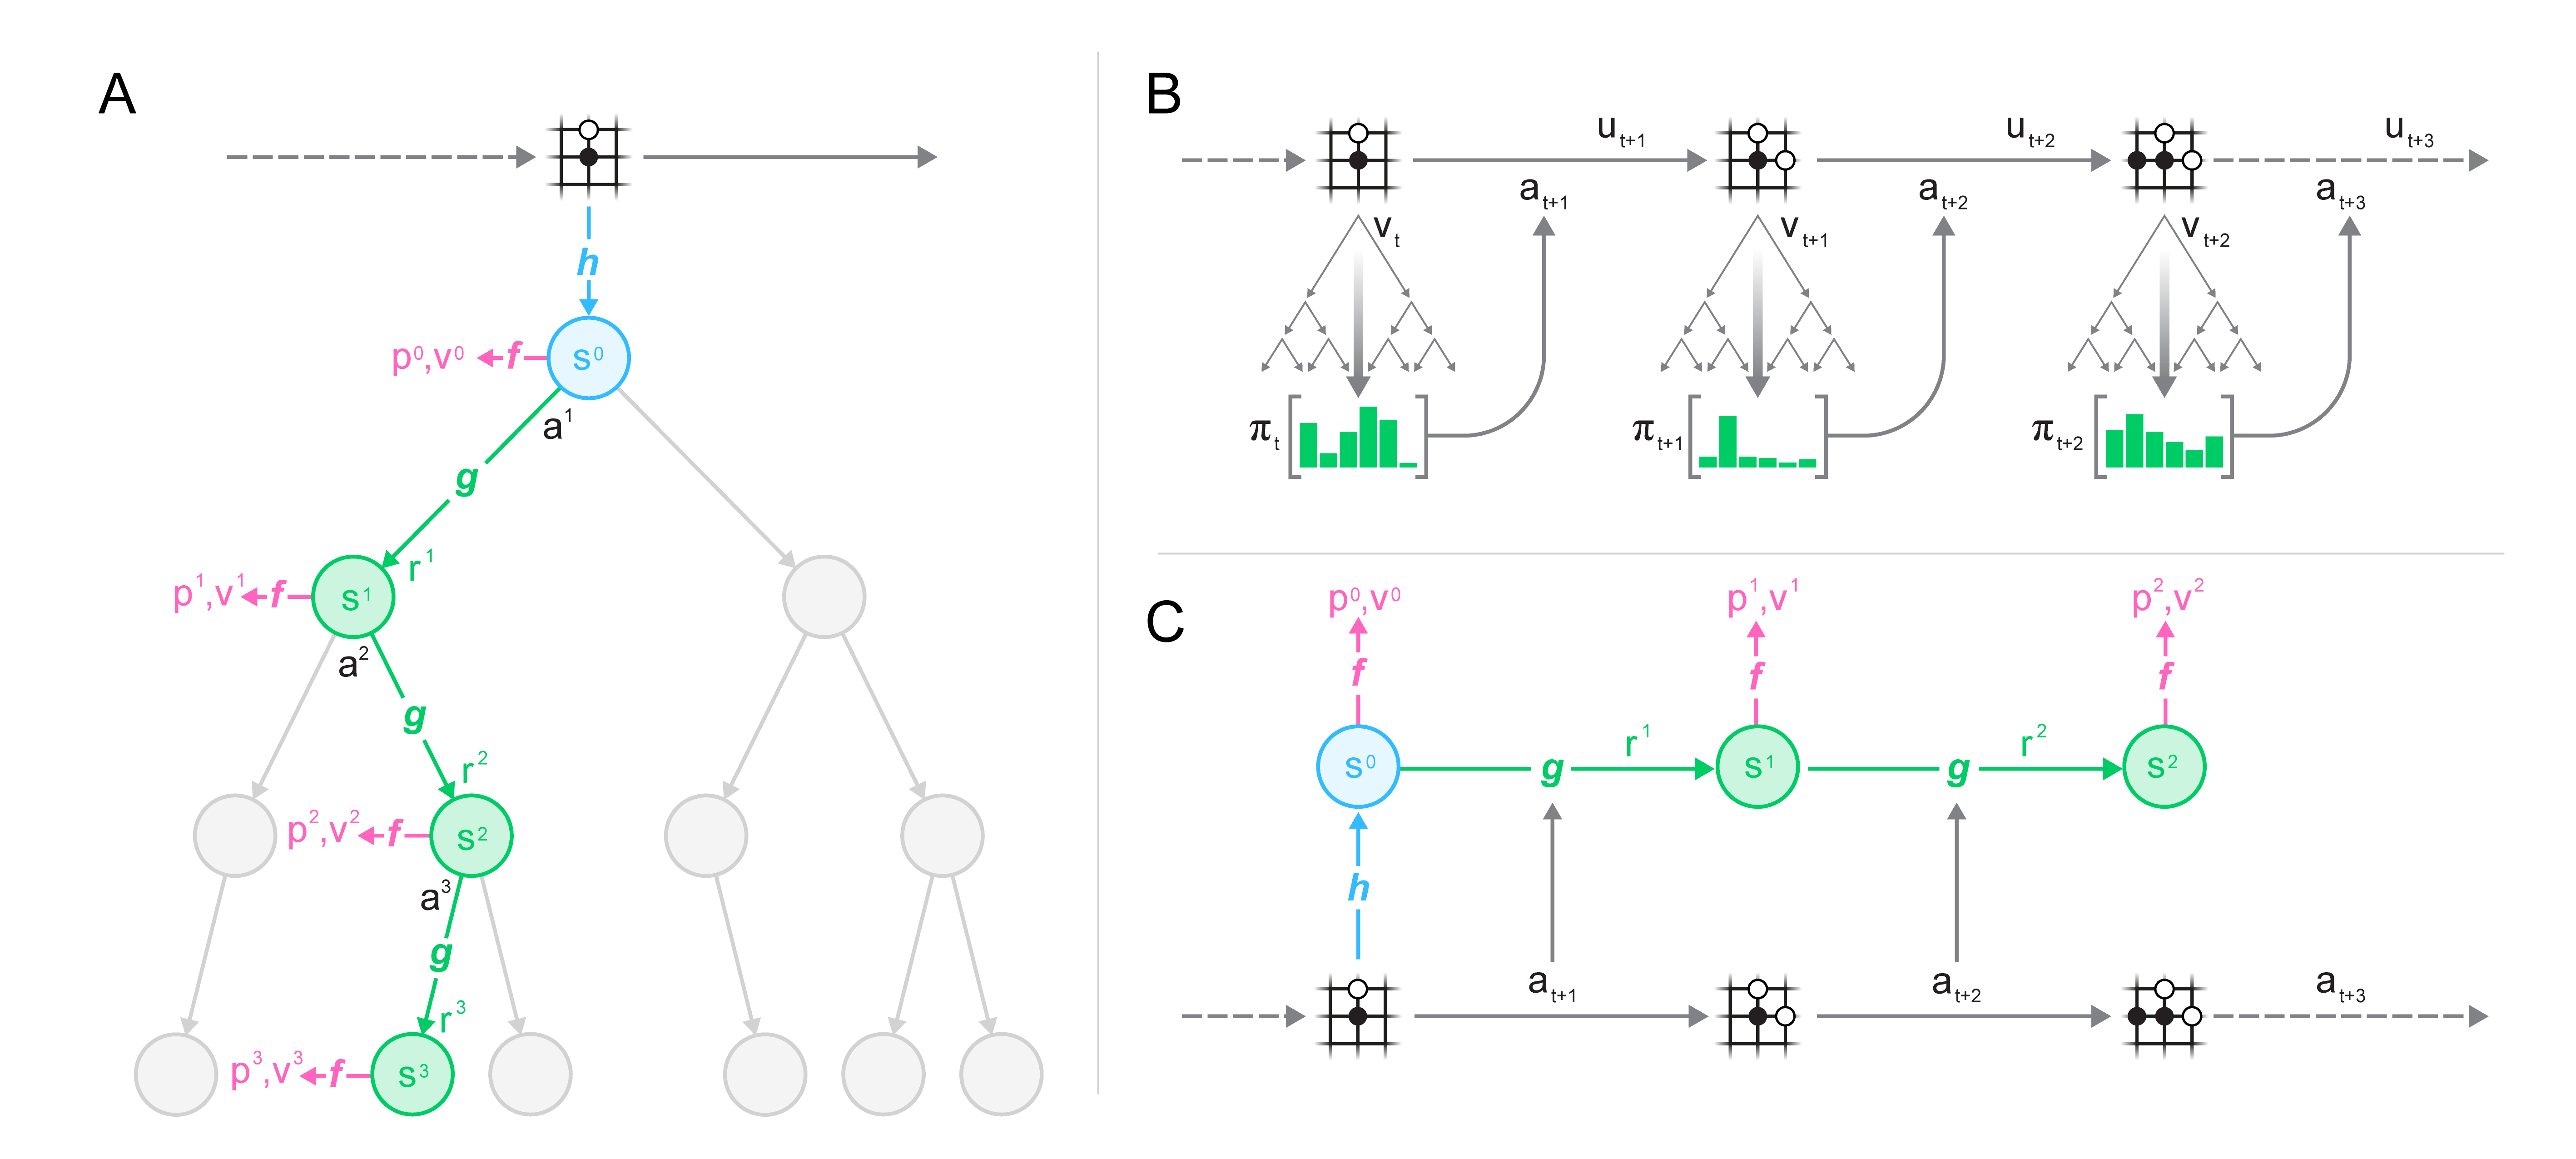
\includegraphics[width=\textwidth]{images/learned_model_search_play_train}
\caption{\label{fig:recurrent_search}
\textbf{使用学习模型进行规划、行动和训练。}
\textbf{(A)} \muzero{} 的模型由表示、动力学和预测三个相互连接的组件组成。给定前一隐藏状态 $s^{k-1}$ 和候选动作 $a^{k}$，\emph{动力学}函数 $g$ 产生即时奖励 $r^{k}$ 和新的隐藏状态 $s^{k}$。策略 $p^k$ 与价值函数 $v^k$ 由\emph{预测}函数 $f$ 从隐藏状态 $s^k$ 计算得到。初始隐藏状态 $s^0$ 由\emph{表示}函数 $h$ 对过去观测（例如围棋棋盘或 Atari 屏幕）编码得到。\textbf{(B)} \muzero{} 如何在环境中行动。每个时间步 $t$ 都执行一次蒙特卡洛树搜索。动作 $a_{t+1}$ 从搜索策略 $\pi_t$ 中采样，该策略与根节点各动作的访问次数成正比。环境接收动作后产生新观测 $o_{t+1}$ 和奖励 $u_{t+1}$。一个回合结束后，轨迹数据被写入重放缓冲区。\textbf{(C)} \muzero{} 如何训练模型。首先从重放缓冲区采样一条轨迹，表示函数 $h$ 接收所选轨迹中的过去观测 $o_1, ..., o_t$。随后模型递归展开 $K$ 步；在每个步骤 $k$，动力学函数 $g$ 以前一步隐藏状态 $s^{k-1}$ 和真实动作 $a_{t+k}$ 为输入。表示、动力学和预测函数的参数通过时间反向传播端到端联合训练，以预测三个量：策略 $\mathbf{p}^k \approx \pi_{t+k}$、价值函数 $v^k \approx z_{t+k}$ 和奖励 $r_{t+k} \approx u_{t+k}$，其中 $z_{t+k}$ 是样本回报，在棋盘游戏中为最终奖励，在 Atari 中为 $n$ 步回报。}
\end{figure}

下面更详细地说明 \muzero{} 算法。在每个时间步 $t$，模型 $\mu_\theta$（参数为 $\theta$）基于过去观测 $o_1, ..., o_t$ 和未来动作 $a_{t+1}, ..., a_{t+k}$，对每个 $k = 1...K$ 的假设步进行预测。模型预测三个未来量：策略 $\mathbf{p}^k_t \approx \pi(a_{t+k+1} | o_1, ..., o_t, a_{t+1}, ..., a_{t+k})$，价值函数 $v^k_t \approx \expect{u_{t+k+1} + \gamma u_{t+k+2} + ... | o_1, ..., o_t, a_{t+1}, ..., a_{t+k}}$，以及即时奖励 $r^k_t \approx u_{t+k}$。其中 $u_{.}$ 表示真实可观测奖励，$\pi$ 是选择真实动作时使用的策略，$\gamma$ 是环境的折扣函数。

在模型内部，每个时间步 $t$（下标 $_t$ 为简洁起见省略）由\emph{表示}函数、\emph{动力学}函数和\emph{预测}函数共同表示。动力学函数 $r^k, s^k = g_\theta(s^{k-1}, a^k)$ 是一个递归过程，在每个假设步骤 $k$ 计算即时奖励 $r^k$ 和内部状态 $s^k$。它在结构上类似于 MDP 模型中给定状态和动作后的期望奖励与状态转移\cite{puterman:MDP}。但与传统基于模型 RL\cite{sutton:book} 不同，内部状态 $s^k$ 不带有环境真实状态的语义。它只是整体模型的隐藏状态，目标是准确预测与未来决策相关的策略、价值和奖励。本文中的\emph{动力学}函数是确定性的；随机转移的扩展留待后续工作。策略和价值由预测函数 $\mathbf{p}^k, v^k = f_\theta(s^k)$ 从内部状态 $s^k$ 计算得到，类似于 \alphazero{} 的联合策略-价值网络。根状态 $s^0$ 由表示函数初始化，即 $s^0 = h_\theta(o_1, ..., o_t)$；除服务于后续预测外，它同样没有额外语义。

有了这样的模型，就可以基于过去观测 $o_1, ..., o_t$ 在假设未来轨迹 $a^1, ..., a^k$ 上进行搜索。例如，一个朴素的搜索可以直接选择使价值函数最大的 $k$ 步动作序列。%
更一般地，可以把任意 MDP 规划算法应用到动力学函数诱导出的内部奖励和状态空间。本文使用一种与 \alphazero{} 搜索相近的 MCTS 算法，并将其推广到单智能体任务和带中间奖励的场景（见“方法”部分）。在每个内部节点，搜索使用当前模型参数 $\theta$ 产生的策略、价值和奖励估计。MCTS 输出推荐策略 $\pi_t$ 和估计价值 $\nu_t$，随后选择动作 $a_{t+1} \sim \pi_t$。

模型的全部参数联合训练，使每个假设步骤 $k$ 的策略、价值和奖励预测，匹配真实时间推进 $k$ 步后观察到的对应目标。与 \alphazero{} 类似，改进后的策略目标由 MCTS 搜索产生；第一个目标是最小化预测策略 $\mathbf{p}_t^k$ 与搜索策略 $\pi_{t+k}$ 之间的误差。改进后的价值目标也来自游戏或 MDP 的实际运行。不同之处在于，\muzero{} 允许长回合、折扣以及中间奖励，因此从未来搜索价值进行 $n$ 步自举：
$z_t = u_{t+1} + \gamma u_{t+2} + ... + \gamma^{n-1} u_{t+n} + \gamma^n \nu_{t+n}$。棋盘游戏中的最终结果 $\{lose, draw, win\}$ 被视为回合最后一步发生的奖励 $u_t \in \{ -1, 0, +1 \}$。第二个目标是最小化预测价值 $v^k_t$ 与价值目标 $z_{t+k}$ 之间的误差\footnote{在国际象棋、围棋和将棋中，奖励与价值使用和 \alphazero{} 相同的平方误差损失。在 Atari 中，奖励和价值的尺度变化较大，实验发现交叉熵损失比平方误差更稳定。两类场景中的策略损失均使用交叉熵。}。奖励目标就是观测到的奖励；因此第三个目标是最小化预测奖励 $r^k_t$ 与观测奖励 $u_{t+k}$ 之间的误差。最后再加入 L2 正则项，得到总体损失：

\begin{align}
l_t(\theta) &= \sum_{k=0}^K l^r (u_{t+k}, r_t^k) + l^v(z_{t+k}, v^k_t) + l^p(\pi_{t+k}, \mathbf{p}^k_t) + c ||\theta||^2
\label{muzero_eqn}
\end{align}
%
其中 $l^r$、$l^v$ 和 $l^p$ 分别为奖励、价值和策略的损失函数。
补充图\ref{fig:muzero_equations} 汇总了 \muzero{} 如何进行规划、行动和学习。

\section{结果}

\begin{figure} %
\begin{tabularx}{\textwidth}{c c c c}

\textbf{国际象棋}
& \textbf{将棋}
& \textbf{围棋}
& \textbf{Atari} \\

\newgame
%
\scalebox{0.62}{\newgame \notationoff \showboard} &
%
\scalebox{0.745}{

\begin{TAB}(e,0.5cm,0.5cm){|c|c|c|c|c|c|c|c|c|}{|c|c|c|c|c|c|c|c|c|}
\rotatebox[origin=c]{180}{香} & \rotatebox[origin=c]{180}{桂} & \rotatebox[origin=c]{180}{銀} & \rotatebox[origin=c]{180}{金} & \rotatebox[origin=c]{180}{玉} & \rotatebox[origin=c]{180}{金} & \rotatebox[origin=c]{180}{銀} & \rotatebox[origin=c]{180}{桂} & \rotatebox[origin=c]{180}{香}\\
 & \rotatebox[origin=c]{180}{飛} & & & & & & \rotatebox[origin=c]{180}{角} & \\
\rotatebox[origin=c]{180}{歩} & \rotatebox[origin=c]{180}{歩} & \rotatebox[origin=c]{180}{歩} & \rotatebox[origin=c]{180}{歩} & \rotatebox[origin=c]{180}{歩} & \rotatebox[origin=c]{180}{歩} & \rotatebox[origin=c]{180}{歩} & \rotatebox[origin=c]{180}{歩} & \rotatebox[origin=c]{180}{歩}\\
 & & & & & & & & \\
 & & & & & & & & \\
 & & & & & & & & \\
歩 & 歩 & 歩 & 歩 & 歩 & 歩 & 歩 & 歩 & 歩\\
 & 角 & & & & & & 飛 & \\
香 & 桂 & 銀 & 金 & 玉 & 金 & 銀 & 桂 & 香\\
\end{TAB}

}%
&
%
\scalebox{0.195}{
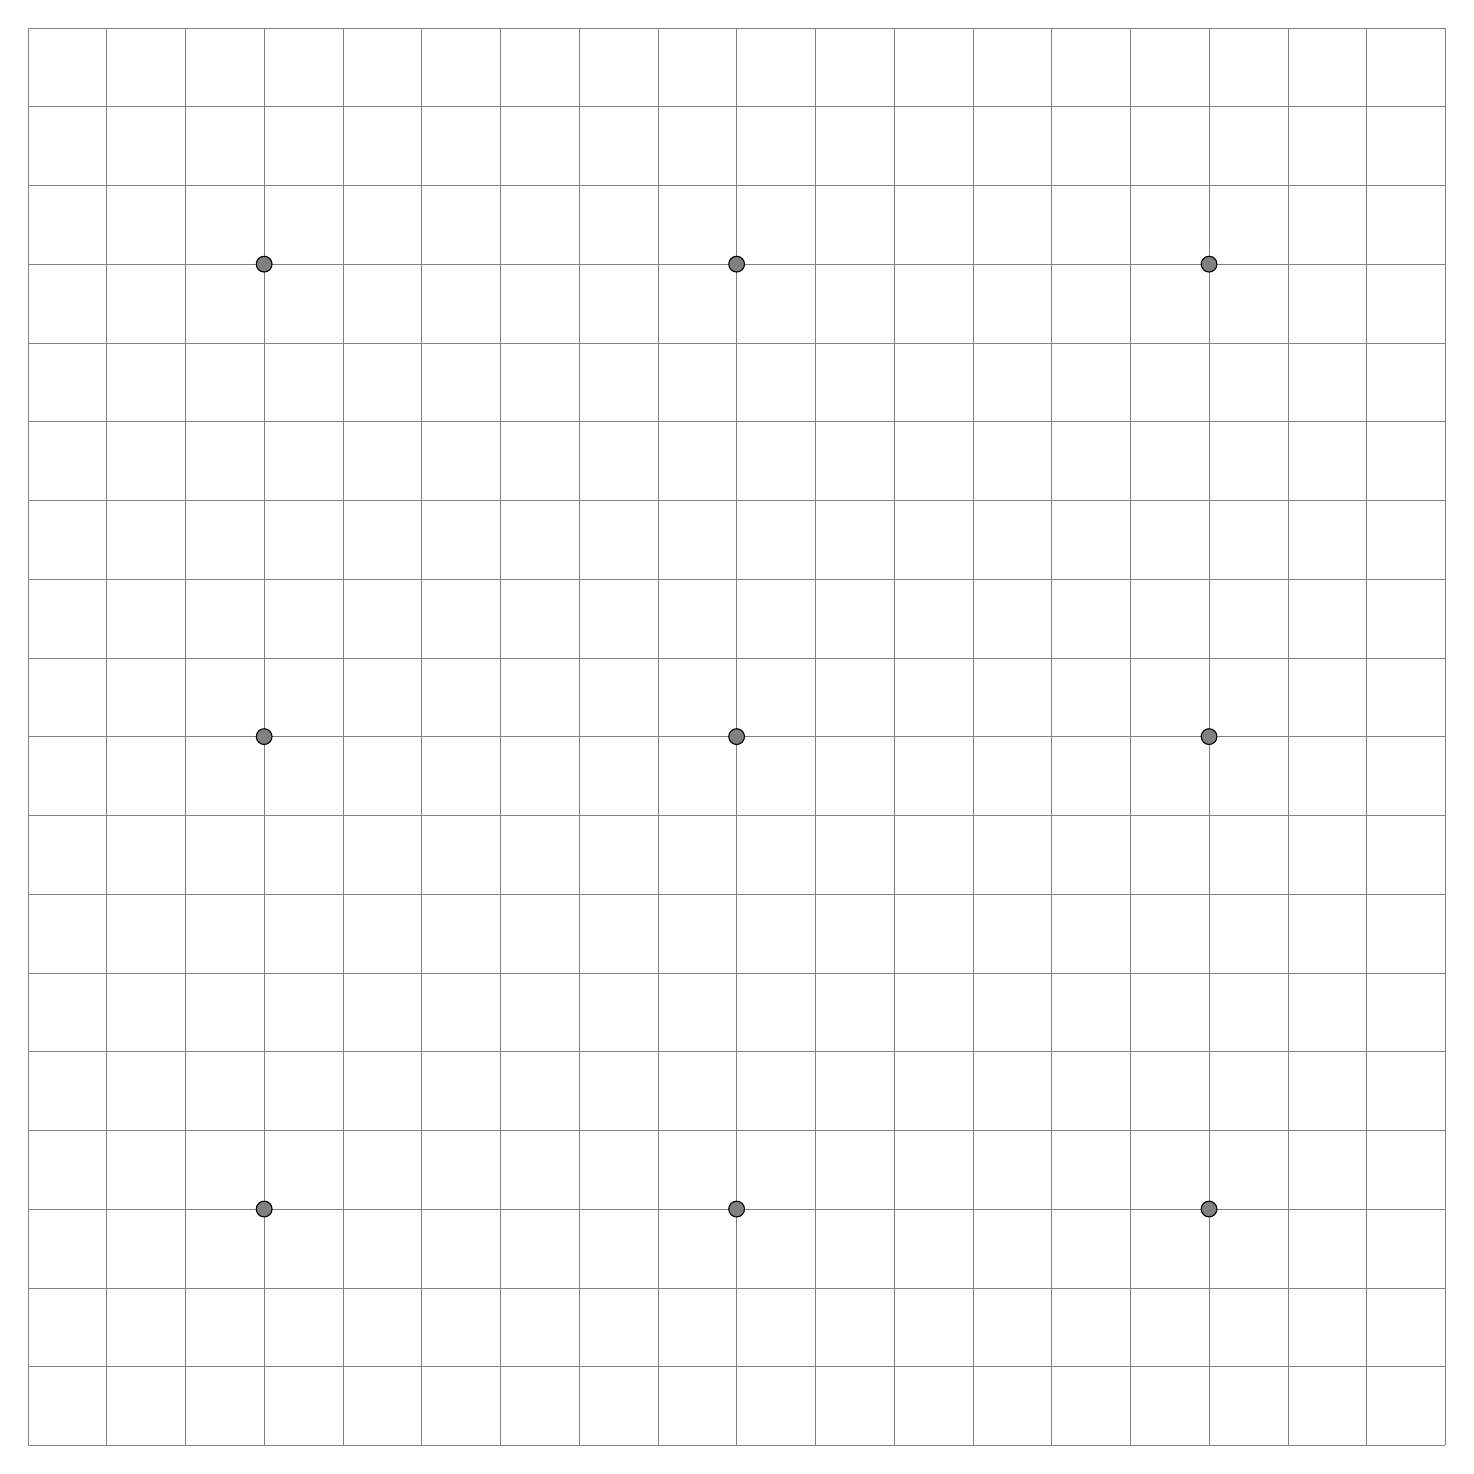
\begin{tikzpicture}
\draw[help lines] (0,0) grid (18,18);
\draw[fill=gray] (3,3) circle[radius=0.1];
\draw[fill=gray] (3,9) circle[radius=0.1];
\draw[fill=gray] (3,15) circle[radius=0.1];
\draw[fill=gray] (9,3) circle[radius=0.1];
\draw[fill=gray] (9,9) circle[radius=0.1];
\draw[fill=gray] (9,15) circle[radius=0.1];
\draw[fill=gray] (15,3) circle[radius=0.1];
\draw[fill=gray] (15,9) circle[radius=0.1];
\draw[fill=gray] (15,15) circle[radius=0.1];
\end{tikzpicture}
}
&
%
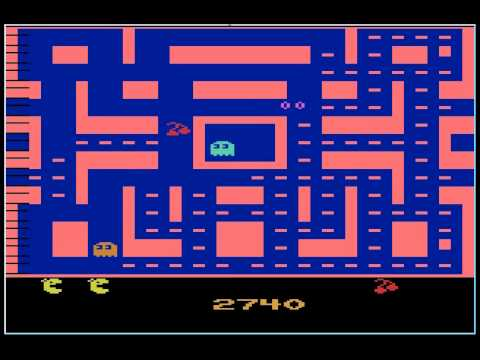
\includegraphics[width=0.219\textwidth,height=0.219\textwidth]{images/mspacman}
\\

\multicolumn{4}{c}{
 \hspace{-3.25em}
 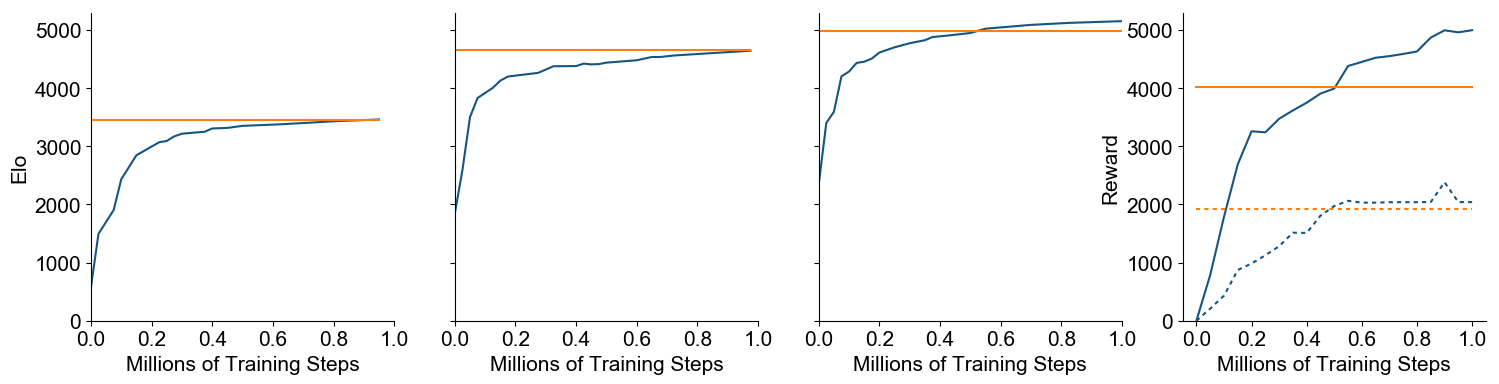
\includegraphics[width=\textwidth + 2.6em]{generated/training_plots}
}

\\

\end{tabularx}

\caption{\label{fig:results}
\textbf{\muzero{} 在国际象棋、将棋、围棋和 Atari 训练过程中的评估结果。} 横轴为百万级训练步数。对于国际象棋、将棋和围棋，纵轴为 Elo 等级分，该等级分通过与 \alphazero{} 对弈估计，双方每步均使用 800 次模拟。\muzero{} 的 Elo 用蓝线表示，\alphazero{} 的 Elo 用水平橙线表示。对于 Atari，纵轴显示 57 个游戏上的人类归一化平均分（实线）和中位分（虚线）。R2D2\cite{r2d2} 的分数以水平橙线表示，它是该领域此前基于无模型 RL 的最优方法。Atari 评估中，每 4 个时间步执行一次 50 次模拟，并将选定动作重复 4 次，与既有工作\cite{dqn} 保持一致。}
\end{figure} %

我们将 \muzero{} 应用于经典棋盘游戏围棋、国际象棋和将棋\footnote{扑克等不完美信息博弈并非本文方法直接处理的对象。}，作为高难度规划问题的基准；同时也在 Atari Learning Environment\cite{ALE} 的 57 个游戏上评估，作为视觉复杂 RL 领域的基准。

在所有任务中，我们均将 \muzero{} 展开 $K=5$ 个假设步骤进行训练。棋盘游戏训练 100 万个 mini-batch，每个 batch 大小为 2048；Atari 中 batch 大小为 1024。在训练和评估期间，棋盘游戏每次搜索使用 800 次模拟，Atari 每次搜索使用 50 次模拟。表示函数采用与 \alphazero{} 相同的卷积\cite{convnet} 与残差\cite{he:resnet} 架构，但使用 16 个残差块而非 20 个。动力学函数采用与表示函数相同的架构，预测函数沿用 \alphazero{} 的设计。所有网络均使用 256 个隐藏平面（细节见“方法”部分）。

%

图\ref{fig:results} 展示了各任务在训练过程中的表现。在围棋中，\muzero{} 略微超过 \alphazero{}，尽管它在搜索树每个节点上的计算更少（\muzero{} 每次评估使用 16 个残差块，而 \alphazero{} 使用 20 个）。这说明 \muzero{} 可能把部分计算缓存到了搜索树中，并通过每一次额外应用动力学模型来加深对局面的表示。

在 Atari 中，\muzero{} 在 Arcade Learning Environment 的 57 个游戏上，在人类归一化平均分和中位分两项指标上都达到当时最好的结果。它在 57 个游戏中的 42 个超过此前最优的无模型方法 R2D2\cite{r2d2}，并在所有游戏上超过此前最好的基于模型方法 SimPLe\cite{kaiser:simple}（见表\ref{tab:atari-results-at30}）。

我们还评估了一个更注重样本效率的 \muzero{} 变体。该变体会使用最新网络参数重新运行 MCTS，对旧轨迹进行再分析并生成新的训练目标（见附录\ref{reanalyze}）。在 57 个 Atari 游戏上，每个游戏使用 2 亿帧经验时，\reanalyze{} 的人类归一化中位分达到 731\%，而此前最优无模型方法 IMPALA\cite{impala}、Rainbow\cite{rainbow} 和 LASER\cite{laser} 分别为 192\%、231\% 和 431\%。

\begin{table}

\begin{tabularx}{\textwidth}{c c c c c c}

\toprule
智能体&中位数&平均值&环境帧数&训练时间&训练步数\\
\midrule
Ape-X\cite{apex} & 434.1\% & 1695.6\% & 22.8B &5天& 8.64M\\
R2D2 \cite{r2d2} & 1920.6\% & 4024.9\% & 37.5B &5天时间& 2.16M \\
\muzero{} & \textbf{2041.1\%} & \textbf{4999.2\%} & 20.0B &12小时& 1M \\
\midrule
IMPALA\cite{impala} & 191.8\% & 957.6\% & 200M & -- & -- \\
Rainbow \cite{rainbow} & 231.1\% & -- & 200M &10天时间& -- \\
UNREAL\textsuperscript{a} \cite{unreal} & 250\%\textsuperscript{a} & 880\%\textsuperscript{a} & 250M & -- & -- \\
LASER\cite{laser} & 431\% & -- & 200M & -- & -- \\
\reanalyze{} & \textbf{731.1\%} & \textbf{2168.9\%} & 200M &12小时& 1M \\
\bottomrule
\end{tabularx}

\caption{\label{tab:atari-comparison}
\textbf{\muzero{} 与 Atari 既有智能体的比较。} 我们分别比较大数据设置（表上半部分）和小数据设置（表下半部分）中训练得到的智能体；除 \muzero{} 外，其余智能体均使用无模型 RL 技术。表中给出相对于人类测试者的人类归一化平均分和中位分，最佳结果用\textbf{粗体}标出。\muzero{} 在两种设置中都达到当时最好的结果。\textsuperscript{a} 表示每个游戏单独调节超参数。}
\end{table}

为理解模型在 \muzero{} 中的作用，我们还进行了若干实验，重点考察围棋和 Atari 游戏 Ms.~Pacman。

首先，我们测试规划可扩展性（图\ref{fig:ablations}A）。在围棋这一典型规划问题中，我们比较了使用完美模型搜索的 \alphazero{} 和使用学习模型搜索的 \muzero{}。具体做法是让训练完成的 \alphazero{} 或 \muzero{} 在不同思考时间下运行 MCTS。即使搜索规模远大于训练时的规模（最长 10 秒思考时间，而训练时约为 0.1 秒，另见图\ref{fig:extended_ablations}A），\muzero{} 仍能达到使用完美模型时的表现。

我们也在所有 Atari 游戏上考察了规划的可扩展性（图\ref{fig:ablations}B）。使用训练完成的 \muzero{}，我们比较了不同模拟次数下的 MCTS 表现。与围棋相比，规划在 Atari 中带来的提升较小，可能是因为模型误差更大；性能会随搜索时间略有提高，但大约在 100 次模拟后趋于平台。即便只使用一次模拟，也就是仅按策略网络选择动作，\muzero{} 仍有较好表现。这表明到训练末期，原始策略已经在一定程度上内化了搜索带来的收益（另见图\ref{fig:extended_ablations}B）。

接下来，我们将本文的基于模型学习算法与一个可比的无模型学习算法进行对照（图\ref{fig:ablations}C）。具体而言，我们把 \muzero{} 的训练目标（式\ref{muzero_eqn}）替换为 R2D2 所用的无模型 Q 学习目标，并将价值头和策略头替换为表示 $Q(\cdot|s_t)$ 的单一输出头。随后，我们在不使用搜索的情况下训练并评估该模型。在 Ms.~Pacman 上，这个无模型算法能达到与 R2D2 相同的结果，但学习速度明显慢于 \muzero{}，最终分数也低得多。我们推测，\muzero{} 中基于搜索的策略改进步骤提供了更强的学习信号，而 Q 学习目标通常偏差和方差都较高。

为进一步理解 \muzero{} 的学习机制，我们还测量了训练过程中搜索量对性能的影响。图\ref{fig:ablations}D 显示了在 Ms.~Pacman 中，训练阶段每步使用不同 MCTS 模拟次数时的表现。与此前观察\cite{negative_mcts_results}不同，即便每步只有 6 次模拟，少于动作数量，\muzero{} 仍能学到有效策略并快速提升；模拟次数增加后，性能会进一步跃升。单次迭代中的策略改进分析见图\ref{fig:extended_ablations}C 和 D。

\begin{figure} %
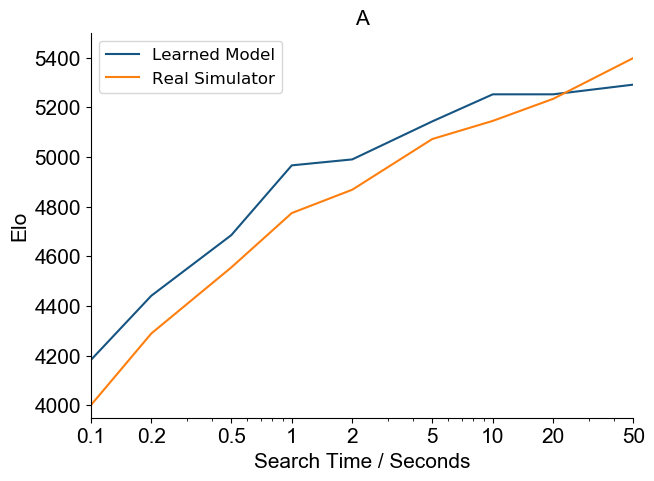
\includegraphics[width=0.5\textwidth]{generated/go_scaling_elos}
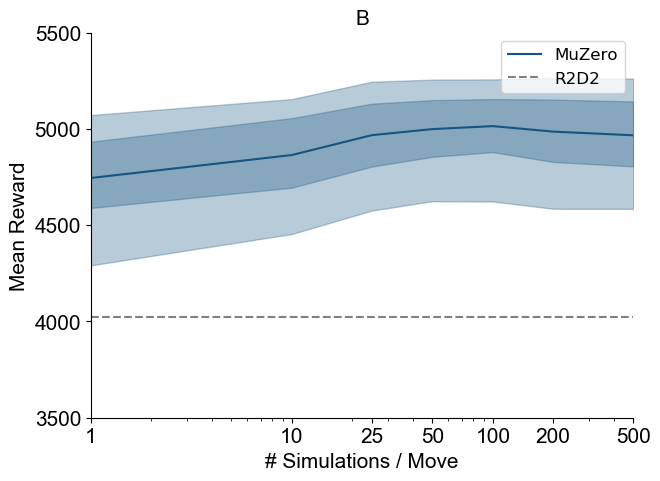
\includegraphics[width=0.5\textwidth]{generated/atari_scaling_score}
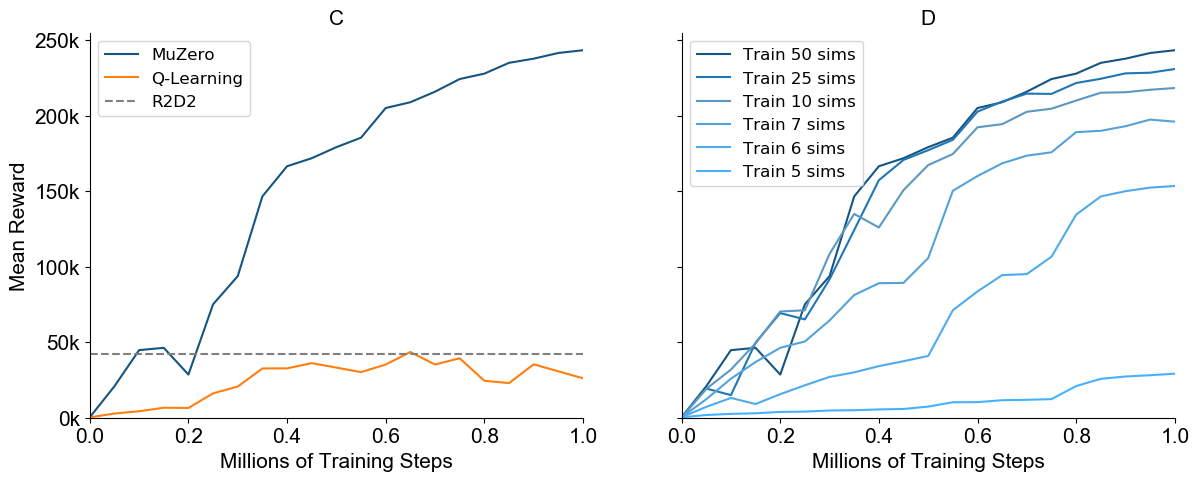
\includegraphics[width=\textwidth]{generated/pacman_ablations_main}
\caption{\label{fig:ablations}
\textbf{\muzero{} 在围棋(A)、57 个 Atari 游戏(B) 和 Ms.~Pacman(C-D) 上的评估。} (\textbf{A}) 围棋中随每步搜索时间扩展的表现，对比学习模型与真实模拟器。两个网络训练时每次搜索均使用 800 次模拟，约等于每次搜索 0.1 秒。学习模型可以扩展到训练时两数量级以上的搜索时间。\textbf{(B)} Atari 最终人类归一化平均分随每次搜索模拟次数的变化。网络训练时每次搜索使用 50 次模拟。深色曲线表示平均分，阴影区域表示第 25--75 百分位和第 5--95 百分位。学习模型的表现随模拟次数增加到约 100 次而提高；继续扩展到远大于训练时的搜索规模后，性能仍保持稳定，仅略有下降。与围棋(A)中更强的扩展性相比，Atari 中的差异可能来自更大的模型误差。\textbf{(C)} 在 \muzero{} 框架内比较基于 MCTS 的训练和 Q 学习，任务为 Ms.~Pacman，并保持网络规模与训练量不变。图中以最优 Q 学习算法 R2D2 作为基线。我们的 Q 学习实现达到与 R2D2 相同的最终分数，但相较基于 MCTS 的训练提升更慢，最终表现也低得多。\textbf{(D)} 不同网络在训练时使用不同的每步模拟次数，但评估时均使用每步 50 次模拟。每步模拟次数更多的网络提升更快，这与(B)中“模拟越多，策略改进越大”的结果一致。即便训练时每步模拟次数少于 Ms.~Pacman 的 8 个可能动作，\muzero{} 仍能有效学习。}
\end{figure} %

\section{结论}

人工智能中的许多结果来自高性能规划\cite{campbell:deep-blue, Silver16AG, Silver18AZ} 或无模型强化学习\cite{dqn, openai_dota, alphastar}。本文提出的方法结合了两者的优势。\muzero{} 在国际象棋和围棋等逻辑复杂的棋盘游戏中达到超越人类水平的表现，同时在视觉复杂的 Atari 游戏中超过最先进的无模型 RL 方法。关键在于，该方法不需要预先知道游戏规则或环境动力学。这说明，学习模型与规划结合后，可以用于缺少完美模拟器的现实世界问题。

\section{致谢}

感谢 Lorrayne Bennett、Oliver Smith 和 Chris Apps 提供组织协助；感谢 Koray Kavukcuoglu 审阅文稿；感谢 Thomas Anthony、Matthew Lai、Nenad Tomasev、Ulrich Paquet 和 Sumedh Ghaisas 参与多次有益讨论；同时感谢 DeepMind 团队其他成员的支持。

%
%

%

%

%
%
%

%
%

\bibliographystyle{plain}
\bibliography{main}

\setcounter{table}{0}
\renewcommand{\thetable}{S\arabic{table}}%
\setcounter{figure}{0}
\renewcommand{\thefigure}{S\arabic{figure}}%

\subsection*{补充材料}

\begin{itemize}
\item 描述 \muzero{} 算法的伪代码。
\item 图\ref{fig:results}、图\ref{fig:ablations}、图\ref{fig:muzero_equations}、图\ref{fig:extended_ablations}、图\ref{fig:learning_curve_atari} 以及表\ref{tab:atari-comparison}、表\ref{tab:atari-results-at30}、表\ref{tab:atari-results-at30-rnd-starts} 对应的 JSON 格式数据。
\end{itemize}

补充材料可从 arXiv 条目的辅助文件部分获取。

\begin{appendices}
\label{methods}


\section{与\alphazero}

\muzero{} 面向比 \alphagozero{}\cite{Silver17AG0} 和 \alphazero{}\cite{Silver18AZ} 更一般的问题设置。

在 \alphagozero{} 和 \alphazero{} 中，规划过程使用两个独立组件：一个执行游戏规则的模拟器，用于在遍历搜索树时更新游戏状态；以及一个神经网络，用于预测模拟器产生的棋盘局面对应的策略和价值（见图\ref{fig:recurrent_search}A）。

具体来说，\alphagozero{} 和 \alphazero{} 在三处使用游戏规则知识：(1) 搜索树中的状态转移，(2) 搜索树每个节点的合法动作，(3) 搜索树内的回合终止。\muzero{} 将这些组件统一替换为由神经网络学习得到的单一隐藏模型（见图\ref{fig:recurrent_search}B）：

\begin{enumerate}[1)]
\item 状态转移。\alphazero{} 使用完美的真实动力学模拟器。\muzero{} 中搜索树的每个节点由一个隐藏状态表示；给定隐藏状态 $s_{k-1}$ 和动作 $a_k$，搜索算法通过 $s_{k} = g(s_{k-1}, a_k)$ 转移到新节点。
\item 合法动作。\alphazero{} 使用模拟器给出的合法动作集合来屏蔽搜索树中每个节点上的网络先验。\muzero{} 只在搜索树根部屏蔽非法动作，因为根部可以查询环境；树内部不再屏蔽。这是可行的，因为网络会很快学到不要预测训练轨迹中从未出现过的动作。
\item 终止节点。\alphazero{} 在表示终止状态的树节点停止搜索，并使用模拟器提供的终局价值，而不是网络输出的价值。\muzero{} 不对终止节点做特殊处理，始终使用网络预测的价值。搜索可以在树内部越过终止节点；此时网络应持续预测相同价值。为此，训练时将终止状态视为吸收状态。
\end{enumerate}

\muzero{} 的目标是在一般强化学习环境中运行，即带有任意尺度折扣中间奖励的单智能体任务。\alphagozero{} 和 \alphazero{} 则主要设计用于双人博弈，且奖励为无折扣的终局 $\pm 1$。

\section{搜索}

下面描述 \muzero{} 的搜索算法。该方法基于带上置信界的蒙特卡洛树搜索，这是一类规划方法；在单智能体任务中，它与最优策略一致，在零和博弈中则与极小极大价值函数一致\cite{kocsis-sepesvari}。

搜索树中的每个节点都关联一个内部状态 $s$。
从 $s$ 出发的每个动作 $a$ 对应一条边 $(s,a)$，该边存储一组统计量
$\{N(s,a), Q(s,a), P(s,a), R(s,a), S(s,a) \}$分别代表访问次数$N$,
平均价值 $Q$、策略先验 $P$、奖励 $R$ 和状态转移 $S$。

与 \alphazero{} 类似，每次搜索由若干次模拟组成，每次模拟分为三个阶段。

\bf 选择：每次模拟从内部根状态 $s^0$ 开始，在到达叶节点 $s^l$ 时结束。
在假设时间步 $k = 1...l$，基于内部状态 $s^{k-1}$ 已存储的统计量，选择使上置信界最大化的动作 $a^k$\cite{rosin:puct,Silver18AZ}：

\begin{equation} \label{pUCT}
a^{k} = \arg\max_{a}\bigg[
Q(s, a) + P(s, a) \cdot \frac{\sqrt{\sum_b N(s, b)}}{1 + N(s, a)} \bigg(c_1 + \log\Big(\frac{\sum_b N(s, b) + c_2 + 1}{c_2}\Big)\bigg) \bigg]
\end{equation}

常数 $c_1$ 和 $c_2$ 控制先验 $P(s, a)$ 相对于价值 $Q(s, a)$ 的影响。在实验中，$c_1 = 1.25$，$c_2 = 19652$。

对于 $k<l$，下一状态和奖励直接从状态转移表与奖励表中读取：$s^{k} = S(s^{k-1}, a^{k})$，$r^{k} = R(s^{k-1}, a^{k})$。

\bf 扩展：在最后的时间步 $l$，奖励和状态由动力学函数计算：$r^l, s^l = g_\theta(s^{l-1}, a^{l})$，
并写入相应表中：$R(s^{l-1}, a^{l}) = r^l, S(s^{l-1}, a^{l}) = s^l$。
策略和价值由预测函数计算：$\mathbf{p}^l, v^l = f_\theta(s^l)$。
状态 $s^l$ 对应的新节点随后加入搜索树。
从新扩展节点出发的每条边 $(s^l, a)$ 初始化为
$\{ N(s^l, a)=0, Q(s^l, a)=0, P(s^l, a)=\mathbf{p}^l \}$.
注意，搜索算法在每次模拟中最多各调用一次动力学函数和预测函数；因此计算成本与 \alphazero{} 相当。

\bf 备份：模拟结束后，沿路径更新统计量。
这里的备份过程适用于环境具有中间奖励、折扣因子 $\gamma$ 不等于 $1$ 且价值估计无固定范围的情形\footnote{在棋盘游戏中，折扣取 $1$，且没有中间奖励。}。
对于 $k = l...0$，我们构造一个 $l-k$ 步的折扣累积奖励估计，并从叶节点价值 $v^l$ 自举：

\begin{equation}
G^k = \sum_{\tau=0}^{l-1-k}{\gamma ^ \tau r_{k+ 1 +\tau}} + \gamma^{l - k} v^l
\end{equation}

对于 $k = l...1$，更新模拟路径中每条边 $(s^{k-1}, a^{k})$ 的统计量：

\begin{equation}
\begin{aligned}
Q(s^{k-1},a^k) & := \frac{N(s^{k-1},a^k) \cdot Q(s^{k-1},a^k) + G^k}{N(s^{k-1},a^k) + 1} \\
N(s^{k-1},a^k) & := N(s^{k-1},a^k) + 1
\end{aligned}
\end{equation}

在双人零和博弈中，通常假设价值函数落在 $[0, 1]$ 区间。这个选择使得式\ref{pUCT} 的 PUCT 规则可以直接结合价值估计和概率。然而，在许多环境中价值没有固定边界，因此需要调整 PUCT 规则。一个简单做法是用环境中可观测的最大分数重新缩放价值，或相应设置 PUCT 常数\cite{MCTS_single_agent}；但这两种做法都依赖具体游戏，并会向 \muzero{} 算法引入额外先验。为避免这一点，\muzero{} 使用搜索树中观察到的最小值和最大值，将 $Q$ 值估计归一化为 $\overline{Q} \in [0, 1]$。当选择阶段到达某个节点时，算法用下式计算边的归一化 $\overline{Q}$，并将其用于 PUCT 规则：

\begin{equation}
\overline{Q}(s^{k-1}, a^k) = \frac{Q(s^{k-1}, a^k) - \min_{s, a \in Tree}Q(s, a)}{\max_{s,a \in Tree} Q(s, a) - \min_{s,a \in Tree} Q(s, a)}
\end{equation}

\section{超参数}

总体上，我们尽量沿用 \alphazero{}\cite{Silver18AZ} 的架构选择和超参数。对于棋盘游戏，我们使用与 \alphazero{} 相同的 UCB 常数、Dirichlet 探索噪声，以及每次搜索 800 次模拟。

Atari 的动作空间更小，策略分布也更紧凑，因此为加速实验，我们每次搜索只使用 50 次模拟。如图\ref{fig:ablations}B 所示，算法对这一选择并不敏感。我们还沿用 R2D2\cite{r2d2} 的折扣因子($0.997$)和值变换（见“网络架构”部分）。

对于文本中没有提到的参数值，请参见伪码。

\section{数据生成}

为生成训练数据，最新网络检查点（每 1000 个训练步更新一次）被用于 MCTS 对弈。在棋盘游戏中，国际象棋和将棋每步使用 800 次模拟来选择动作；在 Atari 中，由于动作空间小得多，每步 50 次模拟即可。

对于棋盘游戏，完整对局结束后即发送给训练任务。Atari 游戏长度更长（最长 30 分钟或 108,000 帧），因此每 200 个动作发送一次中间序列。棋盘游戏训练任务维护一个内置重放缓冲区，保留最近收到的 100 万局游戏；Atari 视觉观测更大，因此保留最近 12.5 万条长度为 200 的序列。

在棋盘游戏中采集经验时，我们使用与 \alphazero{}\cite{Silver18AZ} 相同的探索调度。Atari 中使用该方法的一个变体：整个游戏过程中，动作都从访问次数分布中采样，而不仅限于前 $k$ 步。访问次数分布由温度参数 $T$ 控制：

\begin{equation}
p_{\alpha} = \frac{N(\alpha)^{1 / T}}{\sum_{b} N(b)^{1 / T}}
\end{equation}

$T$ 随网络训练步数衰减。前 500k 步取 $T=1$，接下来的 250k 步取 $T=0.5$，最后 250k 步取 $T=0.25$。这样随着训练推进，动作选择会逐渐变得更贪婪。

\section{网络输入}

\subsection*{表示函数}

对于围棋、国际象棋和将棋，表示函数接收的棋盘状态历史与 \alphazero{}\cite{Silver18AZ} 类似。围棋和将棋中，我们编码过去 8 个棋盘状态；国际象棋中，为正确预测和棋，我们将历史长度增加到最近 100 个棋盘状态。

在 Atari 中，表示函数的输入包括最近 32 帧 RGB 图像（分辨率为 $96 \times 96$），以及导致这些帧出现的最近 32 个动作。我们编码历史动作，是因为与棋盘游戏不同，Atari 中一个动作可能会影响后续多帧观测。RGB 帧按红、绿、蓝三个颜色通道编码，并缩放到 $[0, 1]$ 范围；除此之外，不做额外归一化、白化或预处理。历史动作编码为简单的偏置平面，并按 $a / 18$ 缩放（Atari 中共有 18 个动作）。

\subsection*{动态函数}

动力学函数的输入是表示函数或前一次动力学函数调用产生的隐藏状态，再拼接上转移动作的表示。动作在空间上编码为与隐藏状态同分辨率的平面。Atari 中该分辨率为 $6 \times 6$（见“网络架构”部分的下采样说明）；棋盘游戏中则等于棋盘尺寸（围棋为 $19 \times 19$，国际象棋为 $8 \times 8$，将棋为 $9 \times 9$）。

在围棋中，普通落子动作被编码为一个独热平面，落子位置为 1，其余位置为 0；pass 动作被编码为全零平面。

国际象棋中使用 8 个平面编码动作。第一个独热平面编码被移动棋子的起始位置。接下来的两个平面编码目标位置：若目标在棋盘上，则用一个独热平面表示；另一个二值平面表示目标是否有效（是否在棋盘内）。这样做是因为为简化实现，策略动作空间枚举了所有可能动作，其中并非每个动作都合法；策略预测和动力学函数输入使用同一动作空间。剩余 5 个二值平面表示升变类型（皇后、马、象、车或无升变）。

将棋的编码类似，共使用 11 个平面。前 8 个平面表示棋子从何处移动：要么来自棋盘位置（第一个独热平面），要么是 7 类持驹之一的打入（其余 7 个二值平面）。接下来的两个平面像国际象棋中一样编码目标位置，最后一个二值平面表示该步是否升变。

在 Atari 中，动作被编码为独热向量，并广播为对应的平面。

\section{网络架构}

\label{sec:network_architecture}

预测函数 $\mathbf{p}^k, v^k = f_\theta(s^k)$ 采用与 \alphazero{} 相同的结构：先用一到两层卷积层保持空间分辨率但减少平面数，再接全连接层得到输出。

对于 Atari 的价值和奖励预测，我们沿用 \cite{pohlen2018observe} 的做法，使用可逆变换压缩目标：
$h(x) = sign(x)(\sqrt{|x| + 1} - 1 + \epsilon x)$，实验中 $\epsilon = 0.001$。随后用变换 $\phi$ 将标量表示为离散支持上的等价表示。支持集合大小为 $601$，覆盖从 $-300$ 到 $300$ 的每个整数。在该变换下，每个标量表示为相邻两个支持点的线性组合，因此原值可由 $x = x_{low} * p_{low} + x_{high} * p_{high}$ 还原。例如，目标 $3.7$ 表示为支持点 $3$ 上权重 $0.3$、支持点 $4$ 上权重 $0.7$。网络的价值和奖励输出同样是大小为 $601$ 的 softmax 分布。推理时，先计算对应 softmax 分布下的期望，再通过反向缩放变换得到实际价值和奖励。价值与奖励的缩放和变换对网络可见，但对算法其余部分透明。

表示函数和动力学函数均使用与 \alphazero{} 类似的架构，但采用 16 个而非 20 个残差块\cite{he:resnet}。每个卷积使用 $3 \times 3$ 卷积核和 256 个隐藏平面。

对于 Atari，由于观测空间分辨率较高，表示函数首先使用步幅为 2 的卷积序列降低空间分辨率。具体地说，输入观测大小为 $96 \times 96$，共有 128 个平面（32 个历史帧，每帧 3 个颜色通道，再加上广播成平面的 32 个对应动作），随后按如下方式下采样：

\begin{itemize}
\item 1 个步幅为 2、输出 128 个平面的卷积层，输出分辨率为 $48 \times 48$。
\item 2 个残差块，128 个平面。
\item 1 个步幅为 2、输出 256 个平面的卷积层，输出分辨率为 $24 \times 24$。
\item 3 个残差块，256 个平面。
\item 1 个步幅为 2 的平均池化层，输出分辨率为 $12 \times 12$。
\item 3 个残差块，256 个平面。
\item 1 个步幅为 2 的平均池化层，输出分辨率为 $6 \times 6$。
\end{itemize}

所有操作的核大小均为 $3 \times 3$。

对于动力学函数（始终在 $6 \times 6$ 的下采样分辨率上运行），动作先被编码成图像，再沿平面维度与前一步隐藏状态拼接。


\section{训练}

训练期间，\muzero{} 网络展开 $K$ 个假设步骤，并拟合从 MCTS actor 生成轨迹中采样得到的序列。序列的选择方式是在重放缓冲区任意游戏中采样一个状态，然后从该状态开始展开 $K$ 步。在 Atari 中，样本按优先经验回放\cite{Schaul2016} 抽取，优先级为 $P(i) = \frac{p_i^\alpha}{\sum_k{p_k^\alpha}}$，其中 $p_i = |\nu_i - z_i|$，$\nu$ 为搜索价值，$z$ 为观测到的 $n$ 步回报。为校正优先采样带来的偏差，我们用重要性采样比率 $w_i = (\frac{1}{N} \cdot \frac{1}{P(i)})^\beta$ 缩放损失。所有实验中均设 $\alpha = \beta = 1$。棋盘游戏中的状态则均匀采样。

序列中的每个观测 $o_t$ 都对应一个 MCTS 策略 $\pi_t$、估计价值 $\nu_t$ 和环境奖励 $u_t$。在每个展开步骤 $k$，网络分别计算该步骤的价值、策略和奖励目标损失，并求和得到 \muzero{} 网络的总损失（见式\ref{muzero_eqn}）。在没有中间奖励的棋盘游戏中，我们省略奖励预测损失。棋盘游戏中直接自举到对局结束，等价于预测最终结果；Atari 中则向未来自举 $n=10$ 步。

为使不同展开步上的梯度量级大致相当，我们在两个位置缩放梯度：

\begin{itemize}
\item 将每个输出头的损失按 $\frac{1}{K}$ 缩放，其中 $K$ 为展开步数。这样无论展开多少步，总梯度量级都保持相近。
\item 在动力学函数起始处将梯度按 $\frac{1}{2}$ 缩放，使施加到动力学函数上的总梯度保持稳定。
\end{itemize}

本文所有实验均展开 $K=5$ 步。详细示意见图\ref{fig:recurrent_search}。

为改善学习过程并限制激活范围，我们还将隐藏状态缩放到与动作输入相同的区间($[0, 1]$)：$s_{scaled} = \frac{s - \min(s)}{\max(s) - \min(s)}$。

所有实验均使用第三代 Google Cloud TPU 运行\cite{tpuv3}。每个棋盘游戏使用 16 个 TPU 训练、1000 个 TPU 自我对弈。%
每个 Atari 游戏使用 8 个 TPU 训练、32 个 TPU 自我对弈。%
Atari 中用于行动的 TPU 比例更小，原因是每步模拟次数更少（50 次而非 800 次），且动力学函数相较表示函数规模更小。


\section{重新分析}
\label{reanalyze}

为提高 \muzero{} 的样本效率，我们引入第二个算法变体 \reanalyze{}。\reanalyze{} 会回看过去的时间步，并使用最新模型参数重新执行搜索，从而可能得到质量高于原始搜索的策略。这个新策略在 \muzero{} 训练中被用作 80\% 更新的策略目标。此外，基于较新参数 $\theta^-$ 的目标网络\cite{dqn} $\cdot, v^- = f_{\theta^-}(s^0)$ 被用于提供更新且更稳定的 $n$ 步自举价值目标：
$z_t = u_{t+1} + \gamma u_{t+2} + ... + \gamma^{n-1} u_{t+n} + \gamma^n v^-_{t+n}$。我们还调整了若干超参数，主要是为了增加样本复用并避免价值函数过拟合。具体而言，每个状态抽取 2.0 个样本，而不是 0.1 个；价值目标权重设为 0.25，策略和奖励目标权重仍为 1.0；$n$ 步回报从 $n=10$ 步缩短为 $n=5$ 步。

\section{评价}

在棋盘游戏中，我们通过测量每个玩家的 Elo 等级分来评估 \muzero{} 的相对实力（图\ref{fig:results}）。玩家 $a$ 击败玩家 $b$ 的概率由逻辑函数 $p(a \text{ defeats } b) = (1 + 10^{(c_{\mathrm{elo}} (e(b) - e(a)))})^{-1}$ 估计；等级分 $e(\cdot)$ 使用 \emph{BayesElo} 程序\cite{coulom:bayeselo} 通过贝叶斯逻辑回归计算，标准常数为 $c_{\mathrm{elo}} = 1/400$。

Elo 等级分基于训练期间不同 \muzero{} 迭代与基线玩家之间的锦标赛结果计算，每步使用 800 次模拟。基线玩家分别为 \stockfish{}、\elmo{} 或 \alphazero{}，并使用等价的每步 100ms 搜索时间。基线玩家的 Elo 锚定到公开数值~\cite{Silver18AZ}。

在 Atari 中，我们对每个游戏统计 1000 个 episode 的平均奖励，每个 episode 限制为标准的 30 分钟或 108,000 帧\cite{gorila}；除非另有说明，每步使用 50 次模拟。为减轻 Atari 模拟器确定性的影响，我们采用两种评估策略：30 次 no-op 随机启动和人类启动。前者在每个 episode 开始时，先随机执行 0 到 30 个 no-op 动作，再把控制权交给智能体；后者从人类专家轨迹中采样起始位置，用于初始化 Atari 模拟器，再交由智能体控制\cite{gorila}。

\end{appendices}

\begin{figure} %
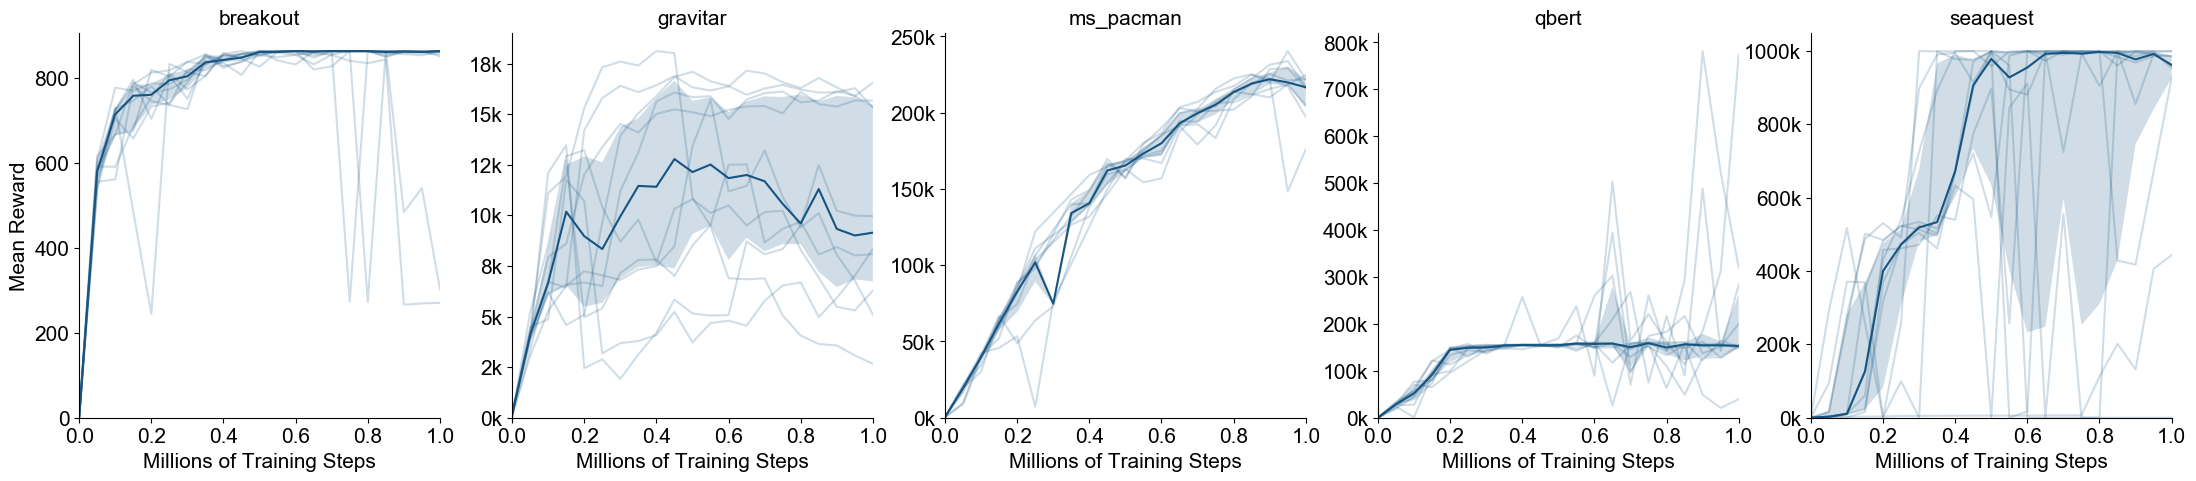
\includegraphics[width=\textwidth]{generated/atari_repeatability.png}
\caption{\label{fig:atari_repeatability}
\textbf{\muzero{} 在五个 Atari 游戏中的可重复性。} 纵轴为总奖励，横轴为百万级训练步数。深色曲线表示 10 次独立训练的中位分，浅色曲线表示单次训练得分，阴影区域表示第 25--75 百分位。}
\end{figure} %

\begin{figure} %

\begin{align*}
&\text{Model} \\
&\left.
\begin{array}{ll}
s^0 &= h_\theta(o_1, ..., o_t) \\
r^k, s^k &= g_\theta(s^{k-1}, a^k) \\
%
\mathbf{p}^k, v^k &= f_\theta(s^k)
\end{array}
\right\} \;\;
\mathbf{p}^k, v^k, r^k = \mu_\theta(o_1, ..., o_t, a^1, ..., a^k)
\end{align*}

\begin{align*}
&\text{Search}\\
\nu_t, \pi_t &= MCTS(s^0_t, \mu_\theta) \\
a_t &\sim \pi_t \\
\\
&\text{Learning Rule} \\
\mathbf{p}^k_t, v^k_t, r^k_t &= \mu_\theta(o_1, ..., o_t, a_{t+1}, ..., a_{t+k}) \\
z_t &= \left\{
\begin{array}{lr}
u_T
& \text{ for games } \\
u_{t+1} + \gamma u_{t+2} + ... + \gamma^{n-1} u_{t+n} + \gamma^n \nu_{t+n}
& \text{ for general MDPs }
\end{array}
\right. \\
l_t(\theta) &= \sum_{k=0}^K l^r (u_{t+k}, r_t^k) + l^v(z_{t+k}, v^k_t) + l^p(\pi_{t+k}, p^k_t) + c ||\theta||^2 \\
\\
&\text{Losses} \\
l^r(u, r) &= \left\{
\begin{array}{lr}
0 & \text{ for games } \\
\boldsymbol{\phi}(u)^T \log \mathbf{r} & \text{ for general MDPs }
\end{array}
\right. \\
l^v(z, q) &= \left\{
\begin{array}{lr}
(z - q)^2 & \text{ for games } \\
\boldsymbol{\phi}(z)^T \log \mathbf{q} & \text{ for general MDPs }
\end{array}
\right. \\
l^p(\pi, p) &= \boldsymbol{\pi}^T \log \mathbf{p}
\end{align*}

\caption{\label{fig:muzero_equations}
\textbf{\muzero{} 算法的公式汇总。} 这里 $\phi(x)$ 表示用相邻整数的线性组合来表示实数 $x$，具体见“网络架构”部分。}
\end{figure} %

\begin{figure} %
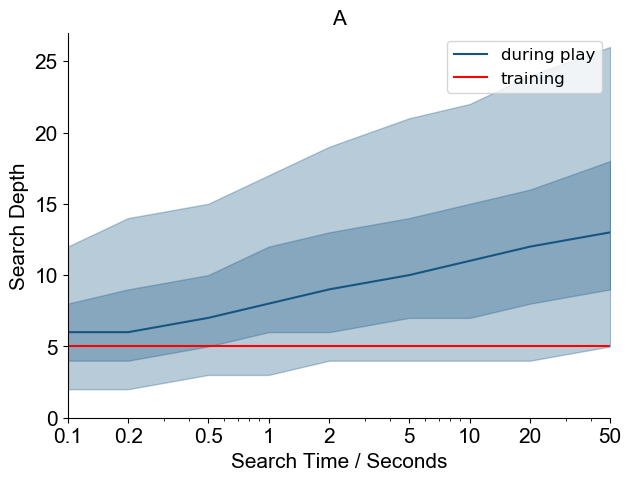
\includegraphics[width=0.5\textwidth]{generated/go_scaling_depth}
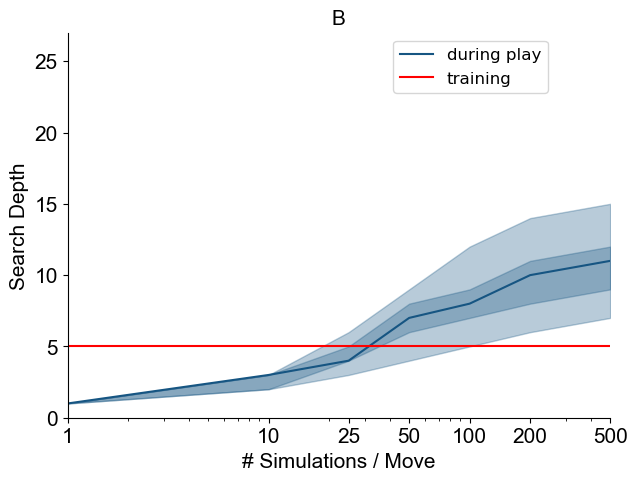
\includegraphics[width=0.5\textwidth]{generated/atari_scaling_depth}
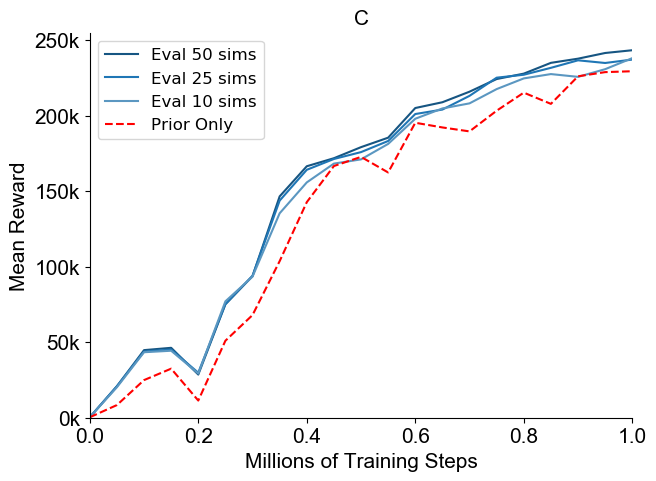
\includegraphics[width=0.5\textwidth]{generated/pacman_ablations_suppl}
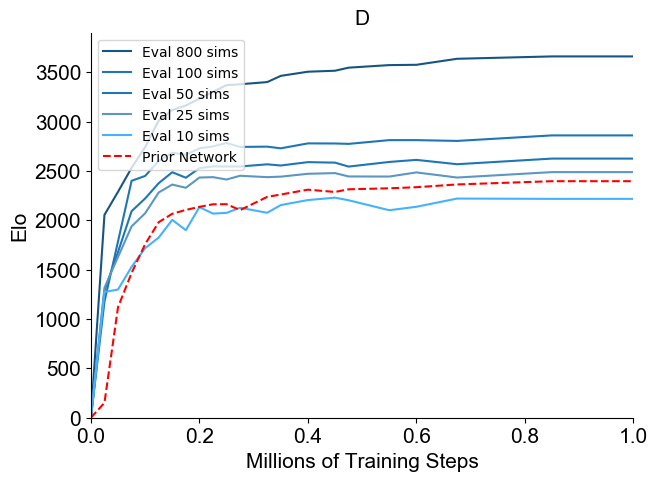
\includegraphics[width=0.5\textwidth]{generated/go_policy_improvement}
\caption{\label{fig:extended_ablations}
\textbf{\muzero{} 评估细节(A-B)与策略改进消融(C-D)。} \textbf{(A-B)} 图\ref{fig:ablations}A-B 中学习模型搜索树的评估深度分布。红线表示网络训练时展开了 5 个假设步骤；深蓝线表示从根节点开始的中位深度，深灰区域为第 25--75 百分位，浅灰区域为第 5--95 百分位。\textbf{(C)} Ms.~Pacman 中的策略改进：单个网络以每次搜索 50 次模拟训练，并在不同模拟次数下评估，包括直接按原始策略网络的 argmax 行动。整个训练过程中，搜索相对于原始策略网络带来的策略改进都清晰可见；有搜索和无搜索之间稳定存在的性能差距，说明 \muzero{} 通过不断向改进后的策略更新来推进学习。\textbf{(D)} 围棋中的策略改进：单个网络以每次搜索 800 次模拟训练，并在不同模拟次数下评估。围棋中，更长搜索带来的棋力提升远大于 Ms.~Pacman，且在整个训练过程中持续存在，这与 \cite{Silver17AG0} 的结果一致，说明模型在精确规划领域的收益更大。}
\end{figure} %

\begin{table}
\scriptsize

\begin{center}\begin{tabularx}{0.900000\textwidth}{X| r r r r r r r}
\toprule
游戏&随机&人类& SimPLe \cite{kaiser:simple} &Ape-X\cite{apex} & R2D2 \cite{r2d2} & \muzero{} & \muzero{} 归一化\\
\midrule
Alien&227.75 & 7,127.80 & 616.90 & 40,805.00 & 229,496.90 & \textbf{741,812.63} & 10,747.5 \%\\
Amidar&5.77 & 1,719.53 & 74.30 & 8,659.00 & \textbf{29,321.40} & 28,634.39 & 1,670.5 \%\\
Assault&222.39 & 742.00 & 527.20 & 24,559.00 & 108,197.00 & \textbf{143,972.03} & 27,664.9 \%\\
Asterix&210.00 & 8,503.33 & 1,128.30 & 313,305.00 & \textbf{999,153.30} & 998,425.00 & 12,036.4 \%\\
Asteroids&719.10 & 47,388.67 & 793.60 & 155,495.00 & 357,867.70 & \textbf{678,558.64} & 1,452.4 \%\\
Atlantis&12,850.00 & 29,028.13 & 20,992.50 & 944,498.00 & 1,620,764.00 & \textbf{1,674,767.20} & 10,272.6 \%\\
Bank Heist&14.20 & 753.13 & 34.20 & 1,716.00 & \textbf{24,235.90} & 1,278.98 & 171.2 \%\\
BattleZone&2,360.00 & 37,187.50 & 4,031.20 & 98,895.00 & 751,880.00 & \textbf{848,623.00} & 2,429.9 \%\\
Beam Rider&363.88 & 16,926.53 & 621.60 & 63,305.00 & 188,257.40 & \textbf{454,993.53} & 2,744.9 \%\\
Berzerk&123.65 & 2,630.42 & - & 57,197.00 & 53,318.70 & \textbf{85,932.60} & 3,423.1 \%\\
Bowling&23.11 & 160.73 & 30.00 & 18.00 & 219.50 & \textbf{260.13} & 172.2 \%\\
Boxing&0.05 & 12.06 & 7.80 & \textbf{100.00} & 98.50 & \textbf{100.00} & 832.2 \%\\
Breakout&1.72 & 30.47 & 16.40 & 801.00 & 837.70 & \textbf{864.00} & 2,999.2 \%\\
Centipede&2,090.87 & 12,017.04 & - & 12,974.00 & 599,140.30 & \textbf{1,159,049.27} & 11,655.6 \%\\
Chopper Command&811.00 & 7,387.80 & 979.40 & 721,851.00 & 986,652.00 & \textbf{991,039.70} & 15,056.4 \%\\
Crazy Climber&10,780.50 & 35,829.41 & 62,583.60 & 320,426.00 & 366,690.70 & \textbf{458,315.40} & 1,786.6 \%\\
Defender&2,874.50 & 18,688.89 & - & 411,944.00 & 665,792.00 & \textbf{839,642.95} & 5,291.2 \%\\
Demon Attack&152.07 & 1,971.00 & 208.10 & 133,086.00 & 140,002.30 & \textbf{143,964.26} & 7,906.4 \%\\
Double Dunk&-18.55 & -16.40 & - & \textbf{24.00} & 23.70 & 23.94 & 1,976.3 \%\\
Enduro&0.00 & 860.53 & - & 2,177.00 & 2,372.70 & \textbf{2,382.44} & 276.9 \%\\
Fishing Derby&-91.71 & -38.80 & -90.70 & 44.00 & 85.80 & \textbf{91.16} & 345.6 \%\\
Freeway&0.01 & 29.60 & 16.70 & \textbf{34.00} & 32.50 & 33.03 & 111.6 \%\\
Frostbite&65.20 & 4,334.67 & 236.90 & 9,329.00 & 315,456.40 & \textbf{631,378.53} & 14,786.7 \%\\
Gopher&257.60 & 2,412.50 & 596.80 & 120,501.00 & 124,776.30 & \textbf{130,345.58} & 6,036.8 \%\\
Gravitar&173.00 & 3,351.43 & 173.40 & 1,599.00 & \textbf{15,680.70} & 6,682.70 & 204.8 \%\\
Hero&1,026.97 & 30,826.38 & 2,656.60 & 31,656.00 & 39,537.10 & \textbf{49,244.11} & 161.8 \%\\
Ice Hockey&-11.15 & 0.88 & -11.60 & 33.00 & \textbf{79.30} & 67.04 & 650.0 \%\\
James Bond&29.00 & 302.80 & 100.50 & 21,323.00 & 25,354.00 & \textbf{41,063.25} & 14,986.9 \%\\
Kangaroo&52.00 & 3,035.00 & 51.20 & 1,416.00 & 14,130.70 & \textbf{16,763.60} & 560.2 \%\\
Krull&1,598.05 & 2,665.53 & 2,204.80 & 11,741.00 & 218,448.10 & \textbf{269,358.27} & 25,083.4 \%\\
Kung-Fu Master&258.50 & 22,736.25 & 14,862.50 & 97,830.00 & \textbf{233,413.30} & 204,824.00 & 910.1 \%\\
Montezuma Revenge&0.00 & \textbf{4,753.33} & - & 2,500.00 & 2,061.30 & 0.00 & 0.0 \%\\
Ms Pacman&307.30 & 6,951.60 & 1,480.00 & 11,255.00 & 42,281.70 & \textbf{243,401.10} & 3,658.7 \%\\
Name This Game&2,292.35 & 8,049.00 & 2,420.70 & 25,783.00 & 58,182.70 & \textbf{157,177.85} & 2,690.5 \%\\
Phoenix&761.40 & 7,242.60 & - & 224,491.00 & 864,020.00 & \textbf{955,137.84} & 14,725.3 \%\\
Pitfall&-229.44 & \textbf{6,463.69} & - & -1.00 & 0.00 & 0.00 & 3.4 \%\\
Pong&-20.71 & 14.59 & 12.80 & \textbf{21.00} & \textbf{21.00} & \textbf{21.00} & 118.2 \%\\
Private Eye&24.94 & \textbf{69,571.27} & 35.00 & 50.00 & 5,322.70 & 15,299.98 & 22.0 \%\\
Qbert&163.88 & 13,455.00 & 1,288.80 & 302,391.00 & \textbf{408,850.00} & 72,276.00 & 542.6 \%\\
Riverraid&1,338.50 & 17,118.00 & 1,957.80 & 63,864.00 & 45,632.10 & \textbf{323,417.18} & 2,041.1 \%\\
Road Runner&11.50 & 7,845.00 & 5,640.60 & 222,235.00 & 599,246.70 & \textbf{613,411.80} & 7,830.5 \%\\
Robotank&2.16 & 11.94 & - & 74.00 & 100.40 & \textbf{131.13} & 1,318.7 \%\\
Seaquest&68.40 & 42,054.71 & 683.30 & 392,952.00 & \textbf{999,996.70} & 999,976.52 & 2,381.5 \%\\
Skiing&-17,098.09 & \textbf{-4,336.93} & - & -10,790.00 & -30,021.70 & -29,968.36 & -100.9 \%\\
Solaris&1,236.30 & \textbf{12,326.67} & - & 2,893.00 & 3,787.20 & 56.62 & -10.6 \%\\
Space Invaders&148.03 & 1,668.67 & - & 54,681.00 & 43,223.40 & \textbf{74,335.30} & 4,878.7 \%\\
Star Gunner&664.00 & 10,250.00 & - & 434,343.00 & \textbf{717,344.00} & 549,271.70 & 5,723.0 \%\\
Surround&-9.99 & 6.53 & - & 7.00 & 9.90 & \textbf{9.99} & 120.9 \%\\
Tennis&-23.84 & -8.27 & - & \textbf{24.00} & -0.10 & 0.00 & 153.1 \%\\
Time Pilot&3,568.00 & 5,229.10 & - & 87,085.00 & 445,377.30 & \textbf{476,763.90} & 28,486.9 \%\\
Tutankham&11.43 & 167.59 & - & 273.00 & 395.30 & \textbf{491.48} & 307.4 \%\\
Up N Down&533.40 & 11,693.23 & 3,350.30 & 401,884.00 & 589,226.90 & \textbf{715,545.61} & 6,407.0 \%\\
Venture&0.00 & 1,187.50 & - & 1,813.00 & \textbf{1,970.70} & 0.40 & 0.0 \%\\
Video Pinball&0.00 & 17,667.90 & - & 565,163.00 & \textbf{999,383.20} & 981,791.88 & 5,556.9 \%\\
Wizard Of Wor&563.50 & 4,756.52 & - & 46,204.00 & 144,362.70 & \textbf{197,126.00} & 4,687.9 \%\\
Yars Revenge&3,092.91 & 54,576.93 & 5,664.30 & 148,595.00 & \textbf{995,048.40} & 553,311.46 & 1,068.7 \%\\
Zaxxon&32.50 & 9,173.30 & - & 42,286.00 & 224,910.70 & \textbf{725,853.90} & 7,940.5 \%\\
\midrule
\# 顶级& 0 & 5 & 0 & 5 & 13 & 37\\
\bottomrule
\end{tabularx}
\end{center}


\caption{\label{tab:atari-results-at30}
\textbf{\muzero{} 在 Atari 单个游戏上的评估结果，采用 30 次随机 no-op 启动。} 每个游戏的最佳结果用\textbf{粗体}标出。每个 episode 最长限制为 30 分钟游戏时间（108k 帧）。SimPLe 只在 57 个游戏中的 36 个上评估，缺失结果以“-”表示。人类归一化分数计算为 $s_{normalized} = \frac{s_{agent} - s_{random}}{s_{human} - s_{random}}$。}
\end{table}

\begin{table}
\scriptsize

\begin{center}\begin{tabularx}{0.750000\textwidth}{X| r r r r r}
\toprule
游戏&随机&人类&Ape-X\cite{apex} & \muzero{} & \muzero{} 归一化\\
\midrule
Alien&128.30 & 6,371.30 & 17,732.00 & \textbf{713,387.37} & 11,424.9 \%\\
Amidar&11.79 & 1,540.43 & 1,047.00 & \textbf{26,638.80} & 1,741.9 \%\\
Assault&166.95 & 628.89 & 24,405.00 & \textbf{143,900.58} & 31,115.2 \%\\
Asterix&164.50 & 7,536.00 & 283,180.00 & \textbf{985,801.95} & 13,370.9 \%\\
Asteroids&877.10 & 36,517.30 & 117,303.00 & \textbf{606,971.12} & 1,700.6 \%\\
Atlantis&13,463.00 & 26,575.00 & 918,715.00 & \textbf{1,653,202.50} & 12,505.6 \%\\
Bank Heist&21.70 & 644.50 & \textbf{1,201.00} & 962.11 & 151.0 \%\\
BattleZone&3,560.00 & 33,030.00 & 92,275.00 & \textbf{791,387.00} & 2,673.3 \%\\
Beam Rider&254.56 & 14,961.02 & 72,234.00 & \textbf{419,460.76} & 2,850.5 \%\\
Berzerk&196.10 & 2,237.50 & 55,599.00 & \textbf{87,308.60} & 4,267.3 \%\\
Bowling&35.16 & 146.46 & 30.00 & \textbf{194.03} & 142.7 \%\\
Boxing&-1.46 & 9.61 & \textbf{81.00} & 56.60 & 524.5 \%\\
Breakout&1.77 & 27.86 & 757.00 & \textbf{849.59} & 3,249.6 \%\\
Centipede&1,925.45 & 10,321.89 & 5,712.00 & \textbf{1,138,294.60} & 13,533.9 \%\\
Chopper Command&644.00 & 8,930.00 & 576,602.00 & \textbf{932,370.10} & 11,244.6 \%\\
Crazy Climber&9,337.00 & 32,667.00 & 263,954.00 & \textbf{412,213.90} & 1,726.9 \%\\
Defender&1,965.50 & 14,296.00 & 399,865.00 & \textbf{823,636.00} & 6,663.7 \%\\
Demon Attack&208.25 & 3,442.85 & 133,002.00 & \textbf{143,858.05} & 4,441.0 \%\\
Double Dunk&-15.97 & -14.37 & 22.00 & \textbf{23.12} & 2,443.1 \%\\
Enduro&-81.84 & 740.17 & 2,042.00 & \textbf{2,264.20} & 285.4 \%\\
Fishing Derby&-77.11 & 5.09 & 22.00 & \textbf{57.45} & 163.7 \%\\
Freeway&0.17 & 25.61 & \textbf{29.00} & 28.38 & 110.9 \%\\
Frostbite&90.80 & 4,202.80 & 6,512.00 & \textbf{613,944.04} & 14,928.3 \%\\
Gopher&250.00 & 2,311.00 & 121,168.00 & \textbf{129,218.68} & 6,257.6 \%\\
Gravitar&245.50 & 3,116.00 & 662.00 & \textbf{3,390.65} & 109.6 \%\\
Hero&1,580.30 & 25,839.40 & 26,345.00 & \textbf{44,129.55} & 175.4 \%\\
Ice Hockey&-9.67 & 0.53 & 24.00 & \textbf{52.40} & 608.5 \%\\
James Bond&33.50 & 368.50 & 18,992.00 & \textbf{39,107.20} & 11,663.8 \%\\
Kangaroo&100.00 & 2,739.00 & 578.00 & \textbf{13,210.50} & 496.8 \%\\
Krull&1,151.90 & 2,109.10 & 8,592.00 & \textbf{257,706.70} & 26,802.6 \%\\
Kung-Fu Master&304.00 & 20,786.80 & 72,068.00 & \textbf{174,623.60} & 851.1 \%\\
Montezuma Revenge&25.00 & \textbf{4,182.00} & 1,079.00 & 57.10 & 0.8 \%\\
Ms Pacman&197.80 & 15,375.05 & 6,135.00 & \textbf{230,650.24} & 1,518.4 \%\\
Name This Game&1,747.80 & 6,796.00 & 23,830.00 & \textbf{152,723.62} & 2,990.7 \%\\
Phoenix&1,134.40 & 6,686.20 & 188,789.00 & \textbf{943,255.07} & 16,969.6 \%\\
Pitfall&-348.80 & \textbf{5,998.91} & -273.00 & -801.10 & -7.1 \%\\
Pong&-17.95 & 15.46 & 19.00 & \textbf{19.20} & 111.2 \%\\
Private Eye&662.78 & \textbf{64,169.07} & 865.00 & 5,067.59 & 6.9 \%\\
Qbert&159.38 & 12,085.00 & \textbf{380,152.00} & 39,302.10 & 328.2 \%\\
Riverraid&588.30 & 14,382.20 & 49,983.00 & \textbf{315,353.33} & 2,281.9 \%\\
Road Runner&200.00 & 6,878.00 & 127,112.00 & \textbf{580,445.00} & 8,688.9 \%\\
Robotank&2.42 & 8.94 & 69.00 & \textbf{128.80} & 1,938.3 \%\\
Seaquest&215.50 & 40,425.80 & 377,180.00 & \textbf{997,601.01} & 2,480.4 \%\\
Skiing&-15,287.35 & \textbf{-3,686.58} & -11,359.00 & -29,400.75 & -121.7 \%\\
Solaris&2,047.20 & \textbf{11,032.60} & 3,116.00 & 2,108.08 & 0.7 \%\\
Space Invaders&182.55 & 1,464.90 & 50,699.00 & \textbf{57,450.41} & 4,465.9 \%\\
Star Gunner&697.00 & 9,528.00 & 432,958.00 & \textbf{539,342.70} & 6,099.5 \%\\
Surround&-9.72 & 5.37 & 6.00 & \textbf{8.46} & 120.5 \%\\
Tennis&-21.43 & -6.69 & \textbf{23.00} & -2.30 & 129.8 \%\\
Time Pilot&3,273.00 & 5,650.00 & 71,543.00 & \textbf{405,829.30} & 16,935.5 \%\\
Tutankham&12.74 & 138.30 & 128.00 & \textbf{351.76} & 270.0 \%\\
Up N Down&707.20 & 9,896.10 & 347,912.00 & \textbf{607,807.85} & 6,606.9 \%\\
Venture&18.00 & \textbf{1,039.00} & 936.00 & 21.10 & 0.3 \%\\
Video Pinball&0.00 & 15,641.09 & 873,989.00 & \textbf{970,881.10} & 6,207.2 \%\\
Wizard Of Wor&804.00 & 4,556.00 & 46,897.00 & \textbf{196,279.20} & 5,209.9 \%\\
Yars Revenge&1,476.88 & 47,135.17 & 131,701.00 & \textbf{888,633.84} & 1,943.0 \%\\
Zaxxon&475.00 & 8,443.00 & 37,672.00 & \textbf{592,238.70} & 7,426.8 \%\\
\midrule
\# 顶级& 0 & 6 & 5 & 46\\
\bottomrule
\end{tabularx}
\end{center}


\caption{\label{tab:atari-results-at30-rnd-starts}
\textbf{\muzero{} 在 Atari 单个游戏上的评估结果，采用人类起始位置。} 每个游戏的最佳结果用\textbf{粗体}标出。每个 episode 最长限制为 30 分钟游戏时间（108k 帧）。}
\end{table}

\begin{figure}
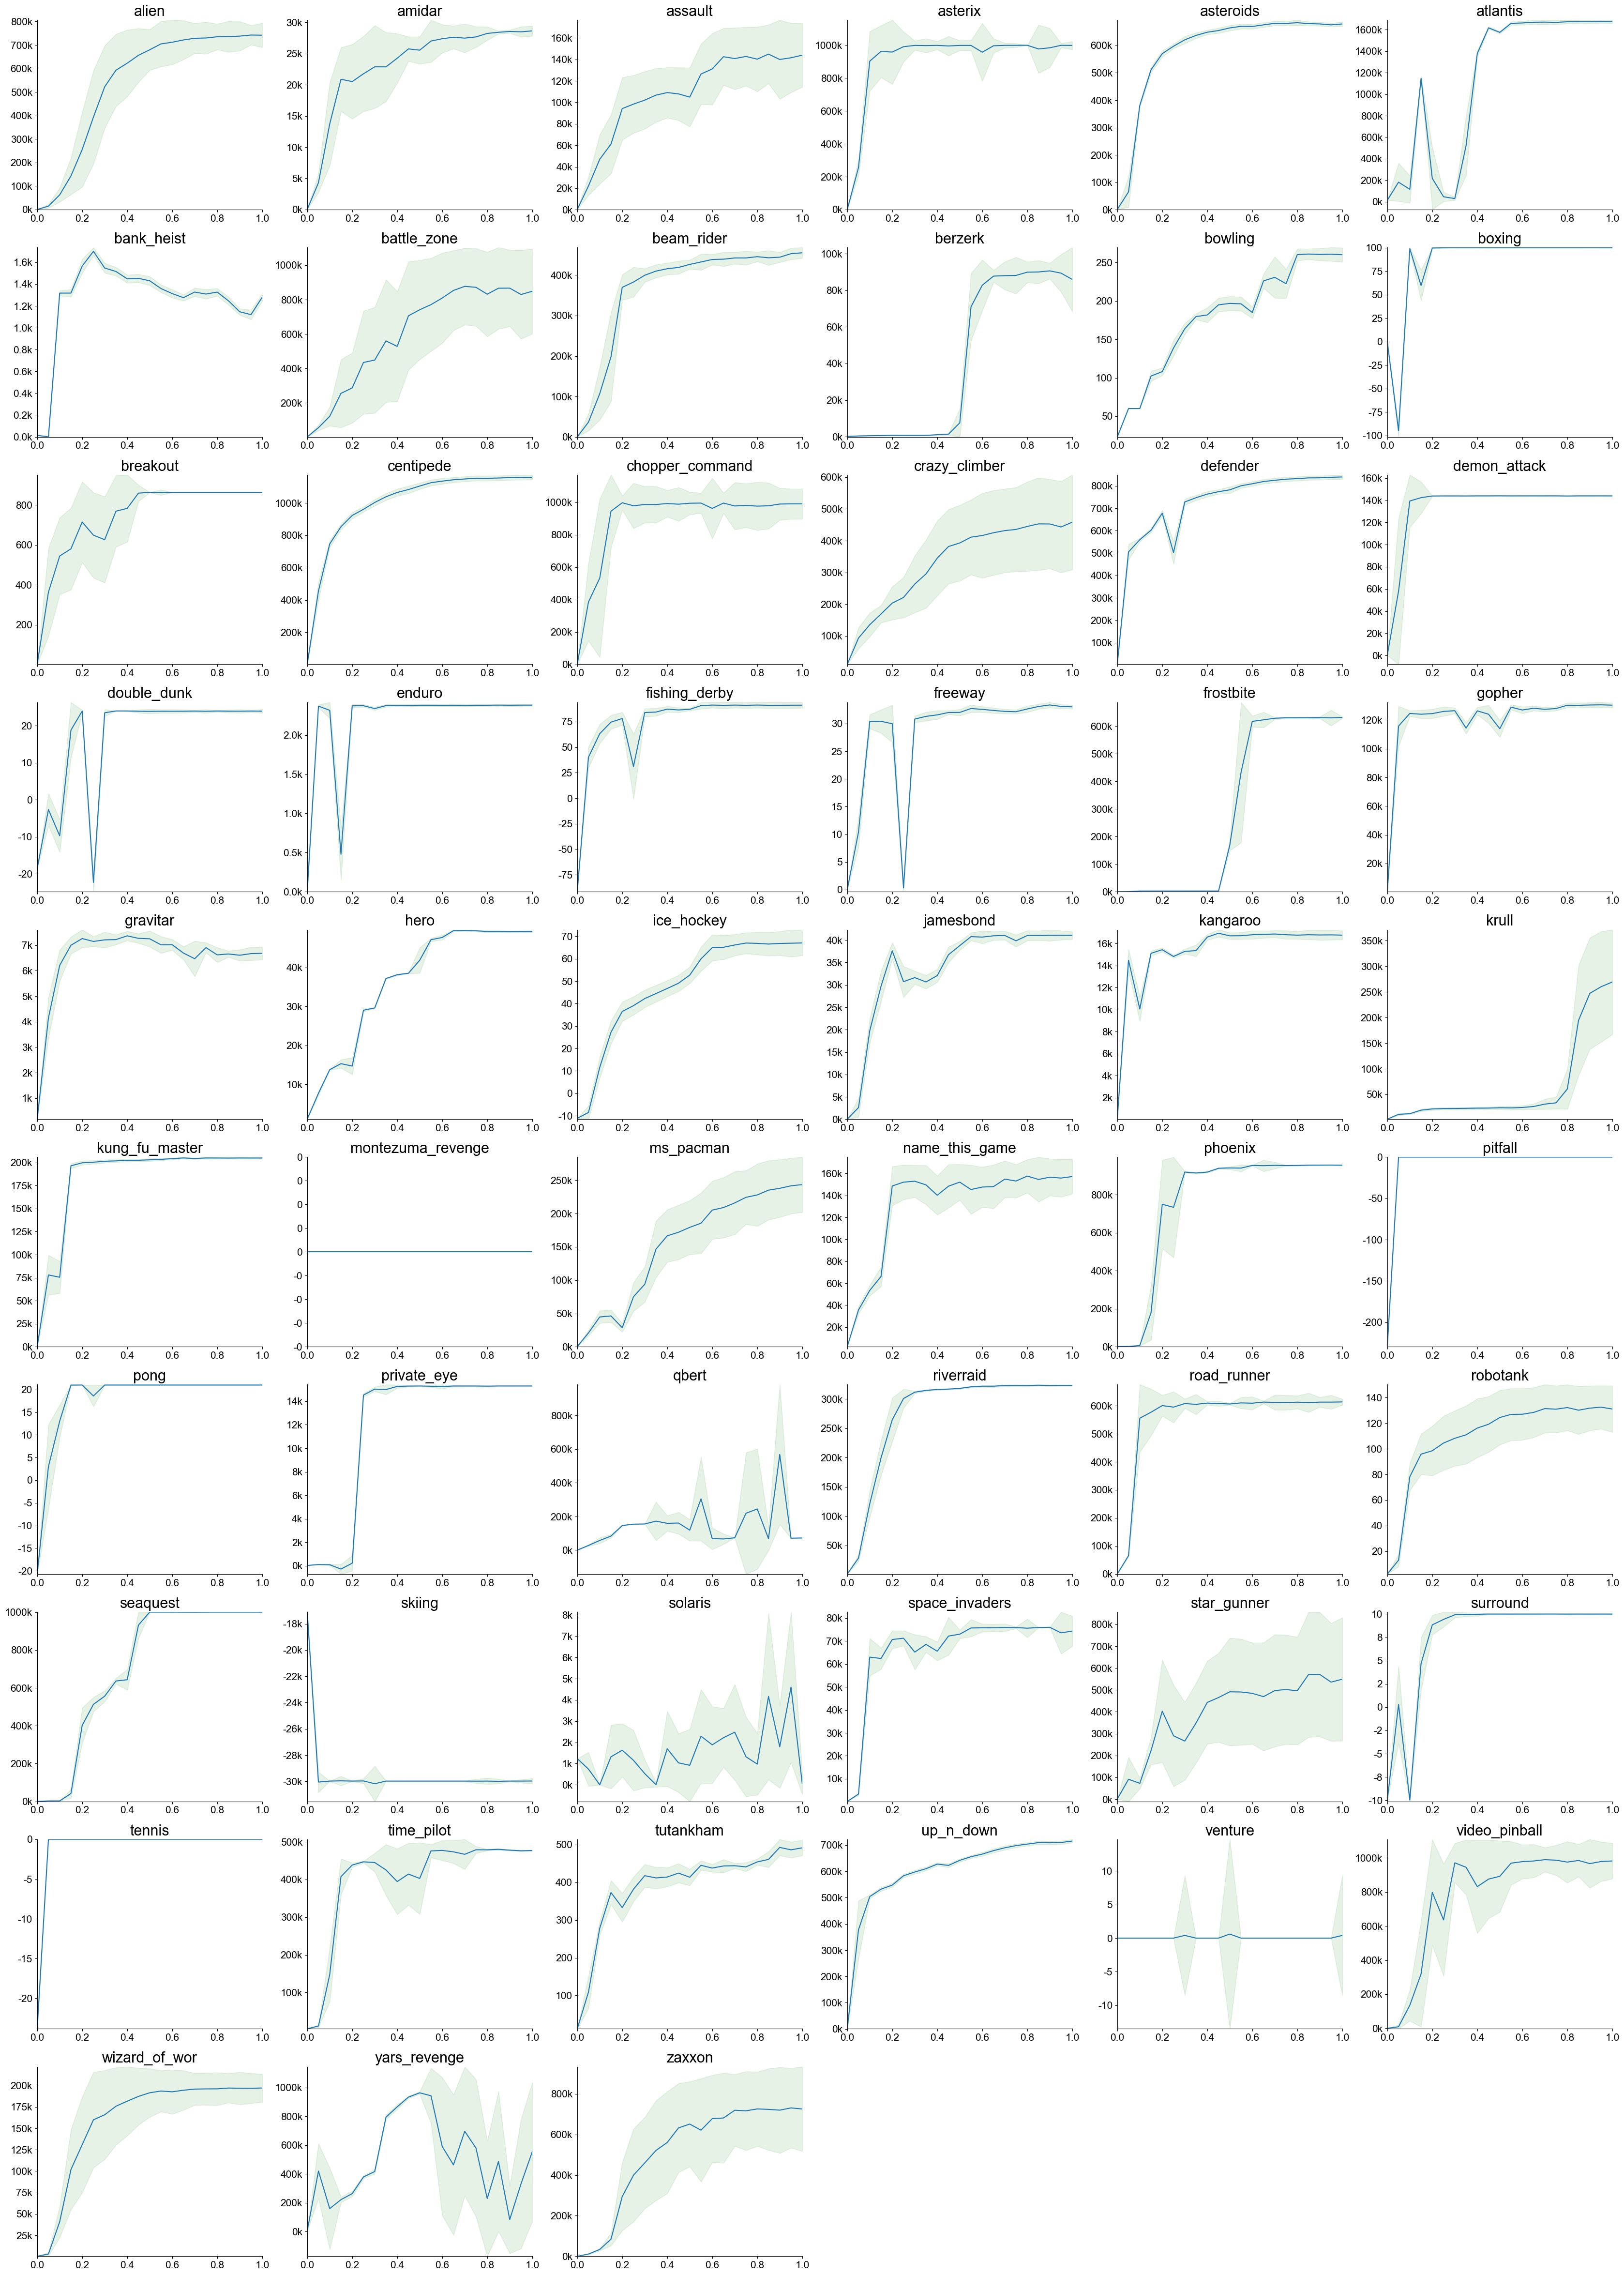
\includegraphics[width=0.95\textwidth]{generated/learning_curve_at30.png}
\caption{\label{fig:learning_curve_atari}
\textbf{\muzero{} 在 Atari 单个游戏上的学习曲线。} 纵轴为总奖励，横轴为百万级训练步数。曲线表示 1000 个评估 episode 的平均分，阴影区域表示标准差。}
\end{figure}

%
%
%
%
%
%
%
%
%
%
%
%
%
%
%
%
%
%
%
%

\end{document}
